% Options for packages loaded elsewhere
\PassOptionsToPackage{unicode}{hyperref}
\PassOptionsToPackage{hyphens}{url}
\PassOptionsToPackage{dvipsnames,svgnames,x11names}{xcolor}
%
\documentclass[
  letterpaper,
  DIV=11,
  numbers=noendperiod,
  oneside]{scrartcl}

\usepackage{amsmath,amssymb}
\usepackage{lmodern}
\usepackage{iftex}
\ifPDFTeX
  \usepackage[T1]{fontenc}
  \usepackage[utf8]{inputenc}
  \usepackage{textcomp} % provide euro and other symbols
\else % if luatex or xetex
  \usepackage{unicode-math}
  \defaultfontfeatures{Scale=MatchLowercase}
  \defaultfontfeatures[\rmfamily]{Ligatures=TeX,Scale=1}
\fi
% Use upquote if available, for straight quotes in verbatim environments
\IfFileExists{upquote.sty}{\usepackage{upquote}}{}
\IfFileExists{microtype.sty}{% use microtype if available
  \usepackage[]{microtype}
  \UseMicrotypeSet[protrusion]{basicmath} % disable protrusion for tt fonts
}{}
\makeatletter
\@ifundefined{KOMAClassName}{% if non-KOMA class
  \IfFileExists{parskip.sty}{%
    \usepackage{parskip}
  }{% else
    \setlength{\parindent}{0pt}
    \setlength{\parskip}{6pt plus 2pt minus 1pt}}
}{% if KOMA class
  \KOMAoptions{parskip=half}}
\makeatother
\usepackage{xcolor}
\usepackage[left=1in,marginparwidth=2.0666666666667in,textwidth=4.1333333333333in,marginparsep=0.3in]{geometry}
\setlength{\emergencystretch}{3em} % prevent overfull lines
\setcounter{secnumdepth}{-\maxdimen} % remove section numbering
% Make \paragraph and \subparagraph free-standing
\ifx\paragraph\undefined\else
  \let\oldparagraph\paragraph
  \renewcommand{\paragraph}[1]{\oldparagraph{#1}\mbox{}}
\fi
\ifx\subparagraph\undefined\else
  \let\oldsubparagraph\subparagraph
  \renewcommand{\subparagraph}[1]{\oldsubparagraph{#1}\mbox{}}
\fi

\usepackage{color}
\usepackage{fancyvrb}
\newcommand{\VerbBar}{|}
\newcommand{\VERB}{\Verb[commandchars=\\\{\}]}
\DefineVerbatimEnvironment{Highlighting}{Verbatim}{commandchars=\\\{\}}
% Add ',fontsize=\small' for more characters per line
\usepackage{framed}
\definecolor{shadecolor}{RGB}{241,243,245}
\newenvironment{Shaded}{\begin{snugshade}}{\end{snugshade}}
\newcommand{\AlertTok}[1]{\textcolor[rgb]{0.68,0.00,0.00}{#1}}
\newcommand{\AnnotationTok}[1]{\textcolor[rgb]{0.37,0.37,0.37}{#1}}
\newcommand{\AttributeTok}[1]{\textcolor[rgb]{0.40,0.45,0.13}{#1}}
\newcommand{\BaseNTok}[1]{\textcolor[rgb]{0.68,0.00,0.00}{#1}}
\newcommand{\BuiltInTok}[1]{\textcolor[rgb]{0.00,0.23,0.31}{#1}}
\newcommand{\CharTok}[1]{\textcolor[rgb]{0.13,0.47,0.30}{#1}}
\newcommand{\CommentTok}[1]{\textcolor[rgb]{0.37,0.37,0.37}{#1}}
\newcommand{\CommentVarTok}[1]{\textcolor[rgb]{0.37,0.37,0.37}{\textit{#1}}}
\newcommand{\ConstantTok}[1]{\textcolor[rgb]{0.56,0.35,0.01}{#1}}
\newcommand{\ControlFlowTok}[1]{\textcolor[rgb]{0.00,0.23,0.31}{#1}}
\newcommand{\DataTypeTok}[1]{\textcolor[rgb]{0.68,0.00,0.00}{#1}}
\newcommand{\DecValTok}[1]{\textcolor[rgb]{0.68,0.00,0.00}{#1}}
\newcommand{\DocumentationTok}[1]{\textcolor[rgb]{0.37,0.37,0.37}{\textit{#1}}}
\newcommand{\ErrorTok}[1]{\textcolor[rgb]{0.68,0.00,0.00}{#1}}
\newcommand{\ExtensionTok}[1]{\textcolor[rgb]{0.00,0.23,0.31}{#1}}
\newcommand{\FloatTok}[1]{\textcolor[rgb]{0.68,0.00,0.00}{#1}}
\newcommand{\FunctionTok}[1]{\textcolor[rgb]{0.28,0.35,0.67}{#1}}
\newcommand{\ImportTok}[1]{\textcolor[rgb]{0.00,0.46,0.62}{#1}}
\newcommand{\InformationTok}[1]{\textcolor[rgb]{0.37,0.37,0.37}{#1}}
\newcommand{\KeywordTok}[1]{\textcolor[rgb]{0.00,0.23,0.31}{#1}}
\newcommand{\NormalTok}[1]{\textcolor[rgb]{0.00,0.23,0.31}{#1}}
\newcommand{\OperatorTok}[1]{\textcolor[rgb]{0.37,0.37,0.37}{#1}}
\newcommand{\OtherTok}[1]{\textcolor[rgb]{0.00,0.23,0.31}{#1}}
\newcommand{\PreprocessorTok}[1]{\textcolor[rgb]{0.68,0.00,0.00}{#1}}
\newcommand{\RegionMarkerTok}[1]{\textcolor[rgb]{0.00,0.23,0.31}{#1}}
\newcommand{\SpecialCharTok}[1]{\textcolor[rgb]{0.37,0.37,0.37}{#1}}
\newcommand{\SpecialStringTok}[1]{\textcolor[rgb]{0.13,0.47,0.30}{#1}}
\newcommand{\StringTok}[1]{\textcolor[rgb]{0.13,0.47,0.30}{#1}}
\newcommand{\VariableTok}[1]{\textcolor[rgb]{0.07,0.07,0.07}{#1}}
\newcommand{\VerbatimStringTok}[1]{\textcolor[rgb]{0.13,0.47,0.30}{#1}}
\newcommand{\WarningTok}[1]{\textcolor[rgb]{0.37,0.37,0.37}{\textit{#1}}}

\providecommand{\tightlist}{%
  \setlength{\itemsep}{0pt}\setlength{\parskip}{0pt}}\usepackage{longtable,booktabs,array}
\usepackage{calc} % for calculating minipage widths
% Correct order of tables after \paragraph or \subparagraph
\usepackage{etoolbox}
\makeatletter
\patchcmd\longtable{\par}{\if@noskipsec\mbox{}\fi\par}{}{}
\makeatother
% Allow footnotes in longtable head/foot
\IfFileExists{footnotehyper.sty}{\usepackage{footnotehyper}}{\usepackage{footnote}}
\makesavenoteenv{longtable}
\usepackage{graphicx}
\makeatletter
\def\maxwidth{\ifdim\Gin@nat@width>\linewidth\linewidth\else\Gin@nat@width\fi}
\def\maxheight{\ifdim\Gin@nat@height>\textheight\textheight\else\Gin@nat@height\fi}
\makeatother
% Scale images if necessary, so that they will not overflow the page
% margins by default, and it is still possible to overwrite the defaults
% using explicit options in \includegraphics[width, height, ...]{}
\setkeys{Gin}{width=\maxwidth,height=\maxheight,keepaspectratio}
% Set default figure placement to htbp
\makeatletter
\def\fps@figure{htbp}
\makeatother

\usepackage{booktabs}
\usepackage{longtable}
\usepackage{array}
\usepackage{multirow}
\usepackage{wrapfig}
\usepackage{float}
\usepackage{colortbl}
\usepackage{pdflscape}
\usepackage{tabu}
\usepackage{threeparttable}
\usepackage{threeparttablex}
\usepackage[normalem]{ulem}
\usepackage{makecell}
\usepackage{xcolor}
\KOMAoption{captions}{tableheading}
\makeatletter
\makeatother
\makeatletter
\@ifpackageloaded{caption}{}{\usepackage{caption}}
\AtBeginDocument{%
\ifdefined\contentsname
  \renewcommand*\contentsname{Table of contents}
\else
  \newcommand\contentsname{Table of contents}
\fi
\ifdefined\listfigurename
  \renewcommand*\listfigurename{List of Figures}
\else
  \newcommand\listfigurename{List of Figures}
\fi
\ifdefined\listtablename
  \renewcommand*\listtablename{List of Tables}
\else
  \newcommand\listtablename{List of Tables}
\fi
\ifdefined\figurename
  \renewcommand*\figurename{Figure}
\else
  \newcommand\figurename{Figure}
\fi
\ifdefined\tablename
  \renewcommand*\tablename{Table}
\else
  \newcommand\tablename{Table}
\fi
}
\@ifpackageloaded{float}{}{\usepackage{float}}
\floatstyle{ruled}
\@ifundefined{c@chapter}{\newfloat{codelisting}{h}{lop}}{\newfloat{codelisting}{h}{lop}[chapter]}
\floatname{codelisting}{Listing}
\newcommand*\listoflistings{\listof{codelisting}{List of Listings}}
\makeatother
\makeatletter
\@ifpackageloaded{caption}{}{\usepackage{caption}}
\@ifpackageloaded{subcaption}{}{\usepackage{subcaption}}
\makeatother
\makeatletter
\@ifpackageloaded{tcolorbox}{}{\usepackage[many]{tcolorbox}}
\makeatother
\makeatletter
\@ifundefined{shadecolor}{\definecolor{shadecolor}{rgb}{.97, .97, .97}}
\makeatother
\makeatletter
\@ifpackageloaded{sidenotes}{}{\usepackage{sidenotes}}
\@ifpackageloaded{marginnote}{}{\usepackage{marginnote}}
\makeatother
\makeatletter
\makeatother
\ifLuaTeX
  \usepackage{selnolig}  % disable illegal ligatures
\fi
\IfFileExists{bookmark.sty}{\usepackage{bookmark}}{\usepackage{hyperref}}
\IfFileExists{xurl.sty}{\usepackage{xurl}}{} % add URL line breaks if available
\urlstyle{same} % disable monospaced font for URLs
\hypersetup{
  colorlinks=true,
  linkcolor={blue},
  filecolor={Maroon},
  citecolor={Blue},
  urlcolor={Blue},
  pdfcreator={LaTeX via pandoc}}

\author{}
\date{}

\begin{document}
\ifdefined\Shaded\renewenvironment{Shaded}{\begin{tcolorbox}[interior hidden, borderline west={3pt}{0pt}{shadecolor}, enhanced, breakable, sharp corners, boxrule=0pt, frame hidden]}{\end{tcolorbox}}\fi

\hypertarget{global-health-research}{%
\section{Global Health Research}\label{global-health-research}}

\begin{Shaded}
\begin{Highlighting}[]
\FunctionTok{library}\NormalTok{(tidyverse)}
\end{Highlighting}
\end{Shaded}

\begin{verbatim}
-- Attaching packages --------------------------------------- tidyverse 1.3.1 --
\end{verbatim}

\begin{verbatim}
v ggplot2 3.3.5     v purrr   0.3.4
v tibble  3.1.6     v dplyr   1.0.8
v tidyr   1.2.0     v stringr 1.4.0
v readr   2.1.2     v forcats 0.5.1
\end{verbatim}

\begin{verbatim}
Warning: package 'tidyr' was built under R version 4.0.5
\end{verbatim}

\begin{verbatim}
Warning: package 'readr' was built under R version 4.0.5
\end{verbatim}

\begin{verbatim}
Warning: package 'dplyr' was built under R version 4.0.5
\end{verbatim}

\begin{verbatim}
-- Conflicts ------------------------------------------ tidyverse_conflicts() --
x dplyr::filter() masks stats::filter()
x dplyr::lag()    masks stats::lag()
\end{verbatim}

\begin{Shaded}
\begin{Highlighting}[]
\FunctionTok{library}\NormalTok{(knitr)}
\FunctionTok{library}\NormalTok{(kableExtra)}
\end{Highlighting}
\end{Shaded}

\begin{verbatim}

Attaching package: 'kableExtra'
\end{verbatim}

\begin{verbatim}
The following object is masked from 'package:dplyr':

    group_rows
\end{verbatim}

\hypertarget{what-is-global-health}{%
\subsection{What is Global Health?}\label{what-is-global-health}}

\emph{New York County Courthouse, Lower Manhattan, New York City, circa
2009}

\textbf{Judge presiding over jury selection:} And what do you do,
Mr.~Green?

\textbf{Me:} Global health research.

\textbf{Judge:}

\textbf{Me:} I study access to mental health services.

\textbf{Judge:} So health policy then?

\textbf{Me:} No, mostly intervention research.

\textbf{Judge}: Globally.

\textbf{Me:} No, not quite.

\textbf{Judge:} What is global health, Mr.~Green?

\textbf{Me:} Well, you see\ldots{}\emph{rambles}\ldots{}

\textbf{Judge:} Thank you, Mr.~Green. You are dismissed.

I've had this conversation hundreds of times since that court
appearance. Now when asked, I say something like, ``global health takes
a global perspective on public health problems,'' drawing inspiration
from @skolnik2019. In the wake of the pandemic, I find that people nod
along at this framing. It makes sense to them. Thanks, COVID-19!

Go any deeper below the ontological surface, however, and you'll find
that there is not a consensus definition of global health
{[}@merson:2018{]}. We'll adopt this one from @koplan:2009:

\begin{quote}
\textbf{Global health is an area for study, research, and practice that
places a priority on improving health and achieving equity in health for
all people worldwide.} Global health emphasizes transnational health
issues, determinants, and solutions; involves many disciplines within
and beyond the health sciences and promotes interdisciplinary
collaboration; and is a synthesis of population-based prevention with
individual-level clinical care.
\end{quote}

Take note of two key elements of their definition:

\begin{enumerate}
\def\labelenumi{\arabic{enumi}.}
\tightlist
\item
  it includes scholars, researchers, and practitioners working across
  disciplinary boundaries; and
\item
  it goes beyond simply improving health to include the goal of
  achieving health equity.
\end{enumerate}

To expand on the first point, this definition reflects the reality that
global health challenges are complex, so the search for solutions must
span disciplines. In the study of malaria, for example, you can read
about the spread of the disease (epidemiology), the impact of illness on
future productivity (economics), the merits of free or subsidized bed
nets (public policy), mosquito habitats (ecology), the efficacy of
vaccines to prevent the disease (medicine and statistics), rapid
diagnostic tests (biomedical engineering), and the adoption and use of
bed nets (psychology), just to name a few areas of inquiry.

The second point is that global health is action-oriented, seeking to
achieve health equity for all people worldwide. The WHO {[}-@who:2021{]}
defines \textbf{equity} as follows:

\begin{quote}
Equity is the absence of unfair, avoidable or remediable differences
among groups of people, whether those groups are defined socially,
economically, demographically, or geographically or by other dimensions
of inequality (e.g.~sex, gender, ethnicity, disability, or sexual
orientation). Health is a fundamental human right. Health equity is
achieved when everyone can attain their full potential for health and
well-being.
\end{quote}

Put another way, health inequities are unfair and unjust differences in
healthcare access or health outcomes that can be prevented or fixed.
Health inequities are structural, often resulting from decisions we make
about who gets access to resources.

The consequence of inequity is often inequality. For instance,
inequitable access to healthcare services can lead to unequal health
outcomes---\textbf{health inequalities}---between groups. Differences in
health status are also referred to as \textbf{health disparities}.

The COVID-19 pandemic has given us many examples of health inequities
and disparities. For instance, data compiled by the website \emph{Health
Inequities Tracker}, visualized in Figure~\ref{fig-disparity}, show that
through at least August 2021, Hispanics and Latinos in the United States
were over-represented in COVID-19 hospitalizations, while non-Hispanic
Whites were substantially under-represented {[}@het{]}.

\begin{Shaded}
\begin{Highlighting}[]
\NormalTok{knitr}\SpecialCharTok{::}\FunctionTok{include\_graphics}\NormalTok{(}\StringTok{"images/figures/disparity.png"}\NormalTok{) }
\end{Highlighting}
\end{Shaded}

\begin{figure*}[H]

{\centering 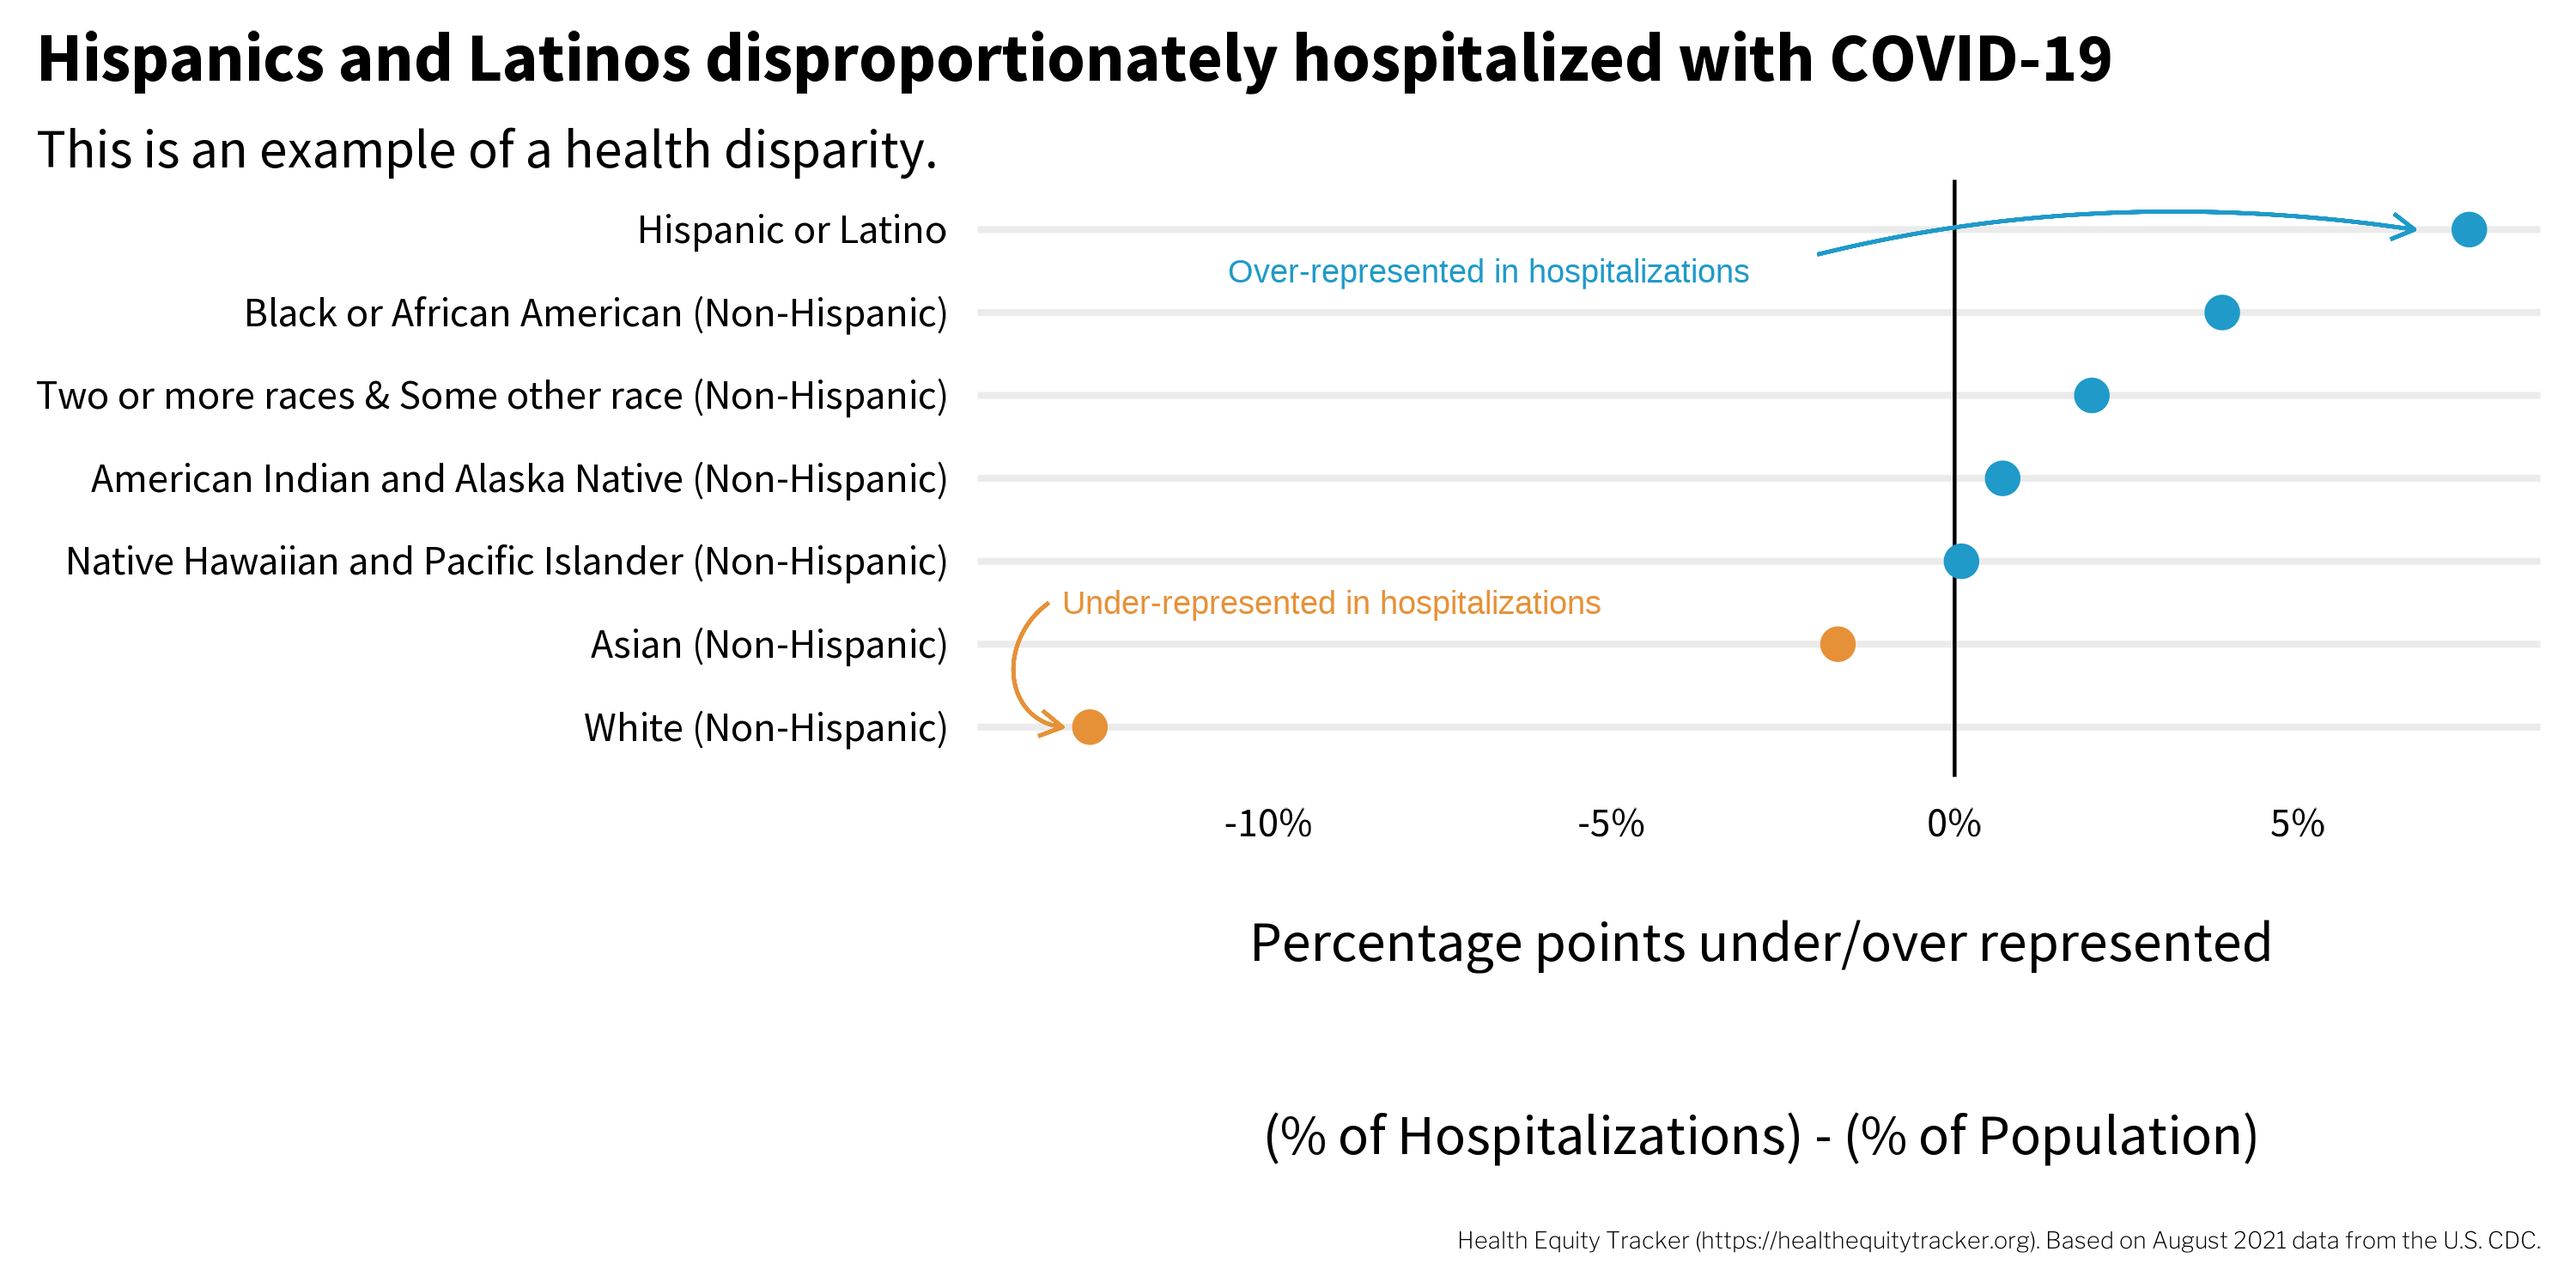
\includegraphics{images/figures/disparity.png}

}

\caption{\label{fig-disparity}COVID-19 health disparities.}

\end{figure*}

@macias:2020 point to several factors that might help to explain why
Latinos and Hispanics were disproportionately affected by COVID-19:

\begin{itemize}
\tightlist
\item
  Higher rates of co-morbid health conditions
\item
  More likely to be underinsured or uninsured
\item
  Undocumented immigration status
\item
  Language barriers to accessing services
\item
  Overrepresentation in ``essential'' jobs where working from home was
  not possible
\item
  Greater financial pressures to show up to work, even if unwell or
  potentially exposed to the virus
\item
  More likely to live in multigenerational homes where transmission was
  more likely
\end{itemize}

Several of these underlying factors, such as undocumented immigration
status, fall into the category of \textbf{social determinants of health}
{[}@who:sd{]}.

\begin{quote}
The circumstances in which people are born, grow up, live, work and age,
and the systems put in place to deal with illness.
\end{quote}

Consider the directed acyclic graph, or DAG, in
Figure~\ref{fig-coviddag} that illustrates how social determinants of
health might have influenced the pandemic. I'll introduce DAGs in more
detail in a later chapter, so for now think of this as a (simplified)
hypothesized conceptual model of what precipitates COVID-19 infection
and hospitalization.

\begin{figure*}

\begin{figure}

{\centering 

\begin{figure}

{\centering 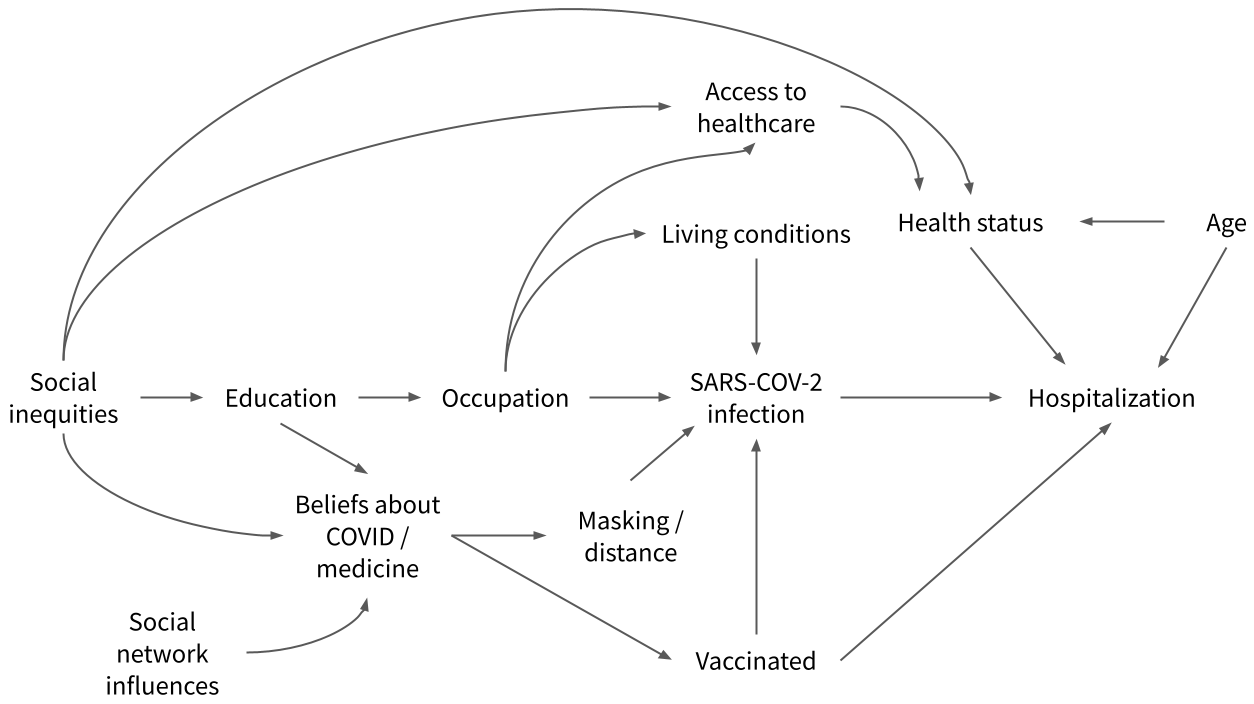
\includegraphics{images/covid_dag.png}

}

\caption{Based on @nafilyan:2021.}

\end{figure}

}

\caption{\label{fig-coviddag}\textbf{?(caption)}}

\end{figure}

\end{figure*}

\begin{figure*}

\begin{Shaded}
\begin{Highlighting}[]
\NormalTok{knitr}\SpecialCharTok{::}\FunctionTok{include\_graphics}\NormalTok{(here}\SpecialCharTok{::}\FunctionTok{here}\NormalTok{(}\StringTok{"images"}\NormalTok{, }\StringTok{"covid\_dag.png"}\NormalTok{)) }
\end{Highlighting}
\end{Shaded}

\end{figure*}

As represented in this DAG, hospitalization with COVID-19 is
\emph{directly} caused by infection with the novel coronavirus,
SARS-CoV-2, but who gets infected is not completely random. Infectious
diseases are social affairs, and some people are more vulnerable because
of their context. For instance, vaccinated individuals are less likely
to get infected, and vaccination rates are highest in the U.S. among the
most educated. Looking further back in the causal chain, educational
attainment is highest among groups without historical social inequities
such as systematic racism.

A diagram like this suggests that to prevent future pandemics we need to
gain a deeper understanding of the interaction between social
determinants of health and disease risk. More importantly, it implies
that we have work to do to fix the underlying societal inequities that
make certain groups more vulnerable. As we've seen with COVID-19,
technological solutions alone---like developing a vaccine in record
time---may not be sufficient.

\begin{Shaded}
\begin{Highlighting}[]
\NormalTok{knitr}\SpecialCharTok{::}\FunctionTok{include\_graphics}\NormalTok{(}\StringTok{"images/covid{-}vaccination{-}doses{-}per{-}capita.png"}\NormalTok{) }
\end{Highlighting}
\end{Shaded}

\begin{figure*}[H]

{\centering 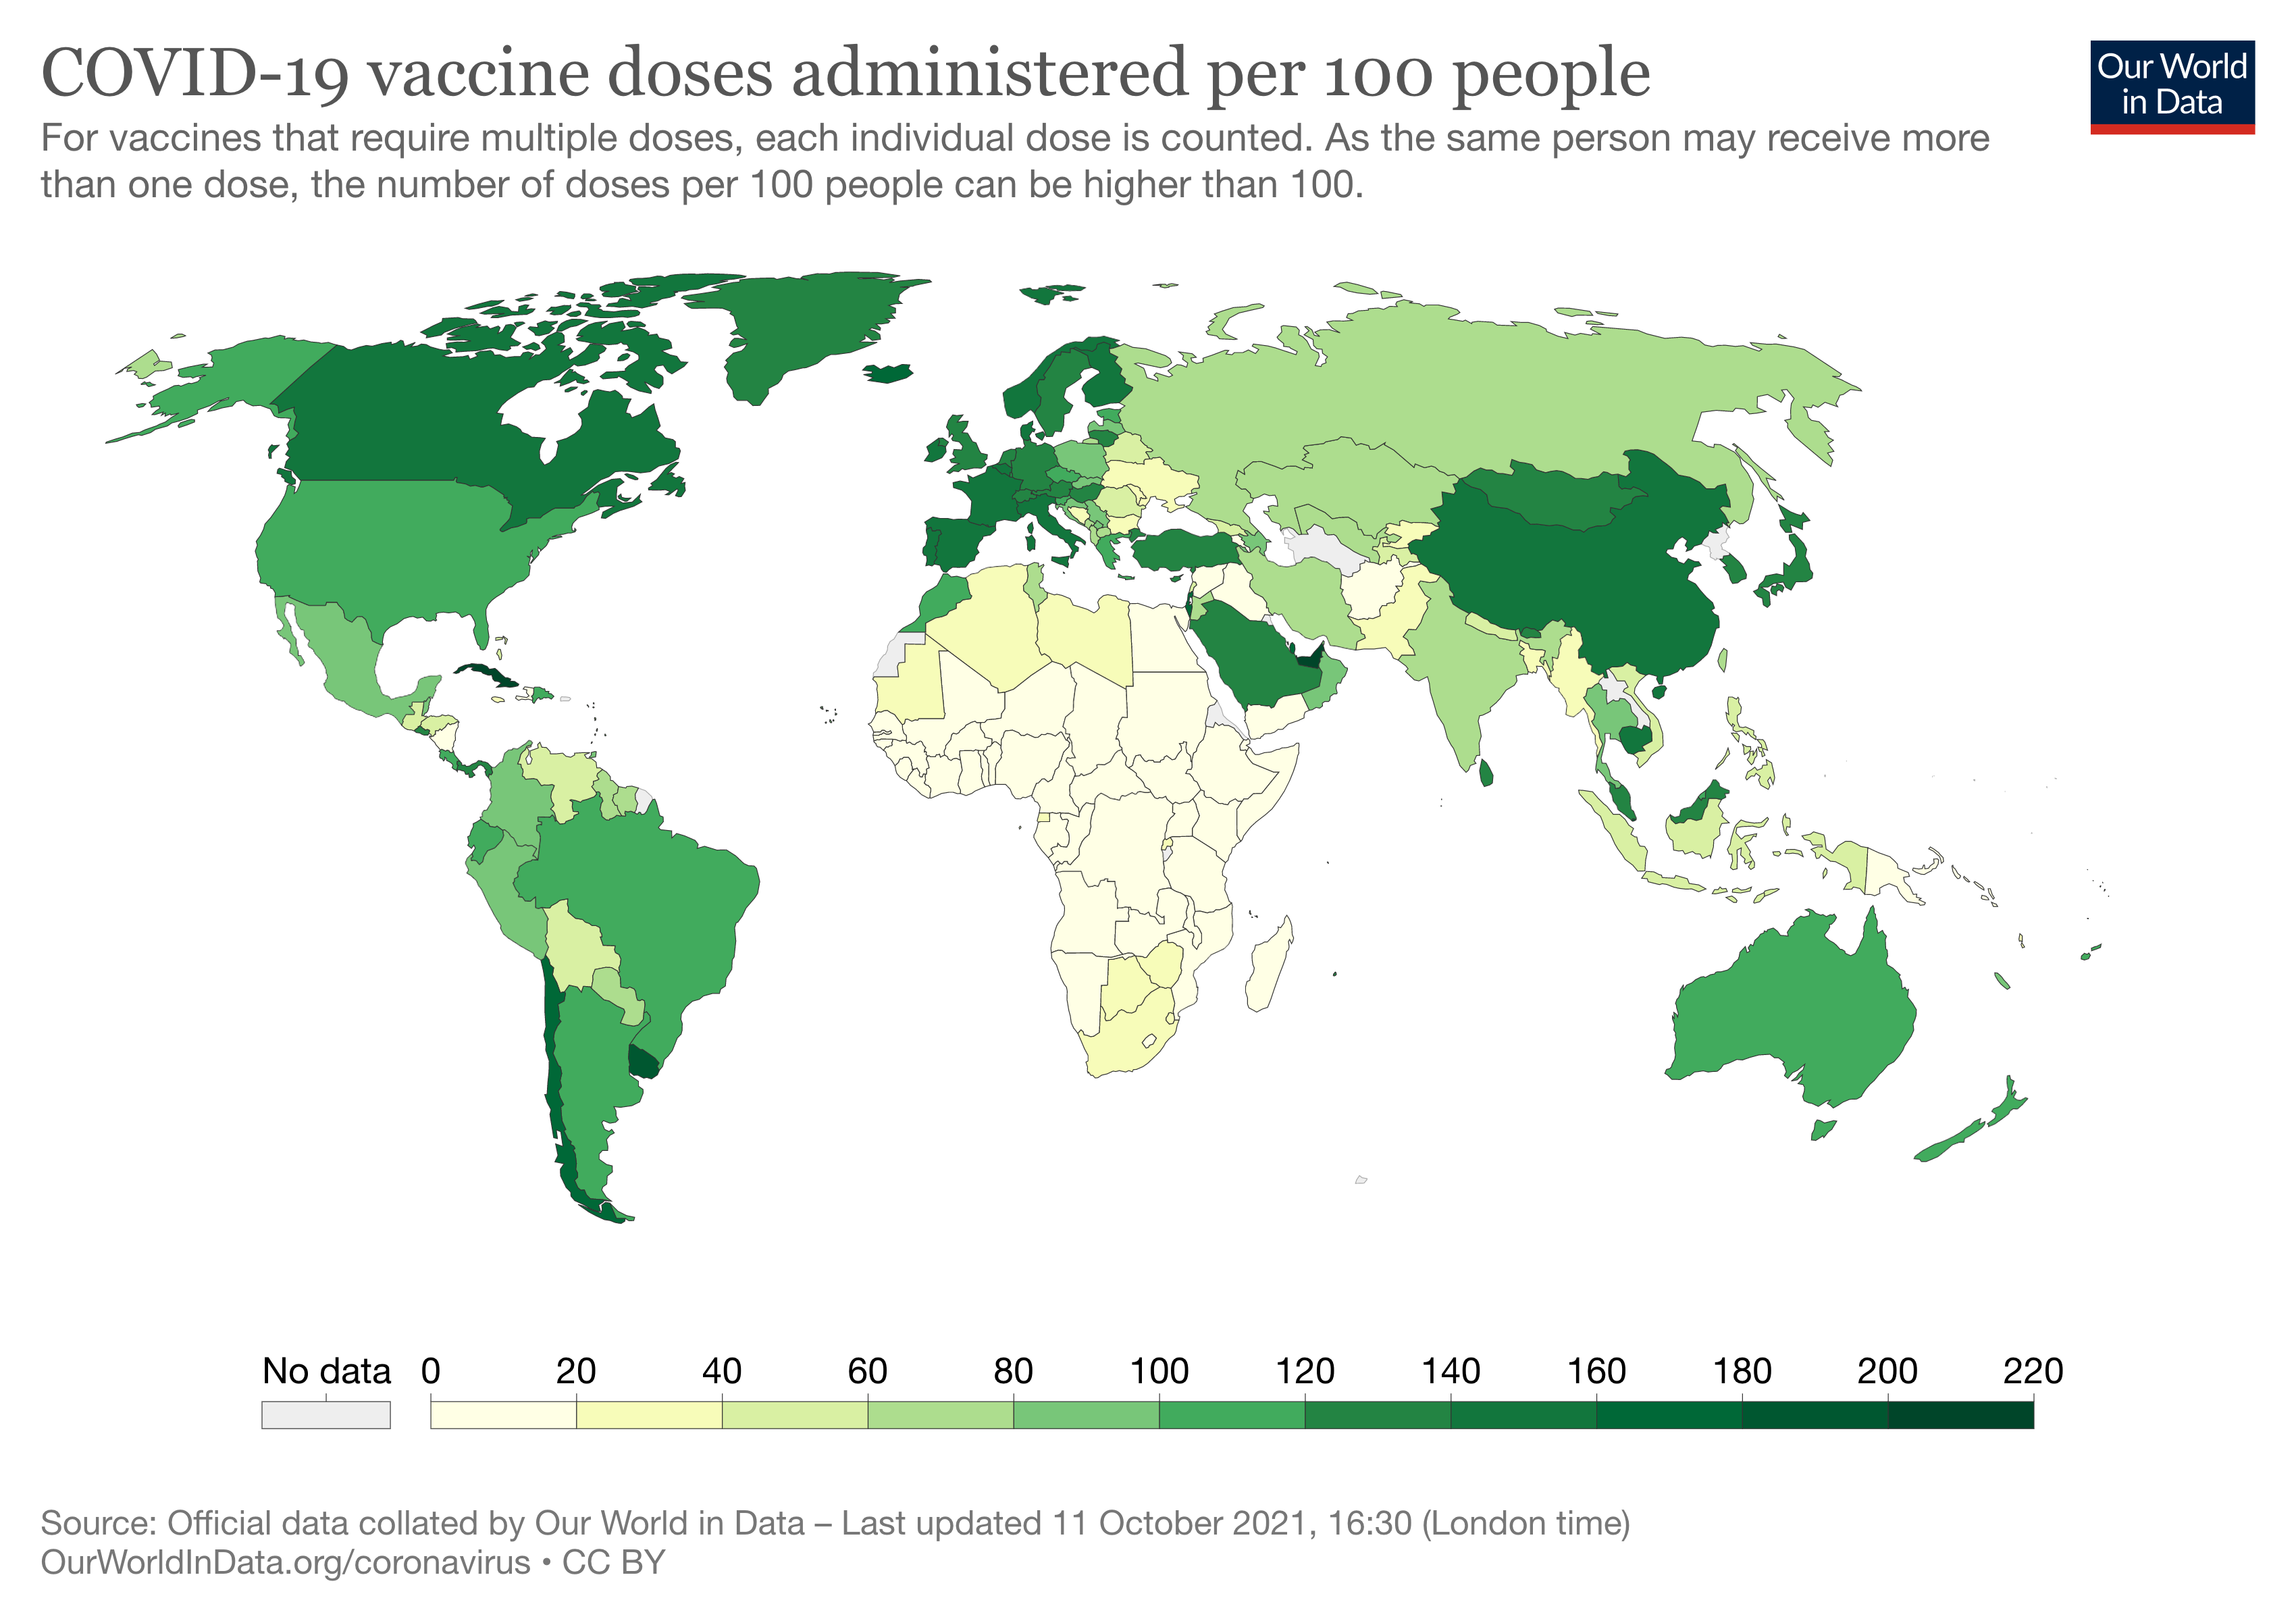
\includegraphics{images/covid-vaccination-doses-per-capita.png}

}

\caption{\label{fig-covidvaccines}Global access to COVID-19 vaccines.}

\end{figure*}

Another example of a COVID-19 inequity is global access to vaccines (see
Figure~\ref{fig-coviddag}. By October 2021, nearly half of the world's
population had received at least one dose of a COVID-19 vaccine, but the
first 6.5 billion doses mostly went into the arms of citizens of wealthy
countries. Less than 3 percent of people in low-income countries had
received even one dose. While true that many low-income countries
escaped the worst of the pandemic's first few waves, the glacial roll
out of vaccines globally---what some have decried as a vaccine
apartheid---leaves many nations vulnerable to deadly new variants. This
puts everyone at risk. Ellen Johnson Sirleaf and Helen Clark, the former
heads of Liberia and New Zealand, respectively, state this plainly in
the inaugural issue of PLOS Global Public Health {[}@sirleaf:2021{]}:

\begin{quote}
Achieving vaccination justice is the first great test of this pandemic
era---it requires targets and aspirations for vaccine access to be
determined by health criteria not a country's economic status, and
timely delivery not a two-speed world where high-income populations are
fully immunized within months but the poor are denied access for years.
Meeting the vaccine justice test will signal that we have both
understood the interdependence that determines our planetary future and
have the capacity to act on it. Failing the test will condemn us to a
`forever crisis' of insecurity and recrimination as virus variants are
given free rein and new vaccines struggle to keep up.
\end{quote}

\hypertarget{what-is-research}{%
\subsection{What is Research?}\label{what-is-research}}

\marginnote{\begin{footnotesize}

\faIcon{book-reader} This definition comes from Title 45 of the United
States Code of Federal Regulations, Part 46, Subpart A, also known as
the Common Rule. Scan the QR code to learn more at
\href{http://ghr.link/shy}{\footnotesize\texttt{ghr.link/shy}}. \newline
\newline

\includegraphics[width=0.78125in,height=\textheight]{images/QR_shy.png}

\end{footnotesize}}

\textbf{Research} is a systematic investigation designed to develop or
contribute to generalizable knowledge. Let's break down this definition.

\begin{enumerate}
\def\labelenumi{\arabic{enumi}.}
\tightlist
\item
  Research is systematic in that it follows a documented and repeatable
  methodology.
\item
  Investigations include research development, testing, and evaluation.
\item
  By generalizable knowledge, we mean that the investigation intends to
  advance our scientific understanding. The goal is to go beyond the
  collection of facts about a particular sample and make conclusions
  that have relevance for other scholars, practitioners, or
  policymakers.
\end{enumerate}

For instance, you might interview parents of young children about their
use of mosquito nets. You intend to analyze the transcripts and develop
new ideas about the barriers to bed net use that you hope to publish in
an academic journal. Other scholars will read this work use it to
develop new theories of health behavior and create new interventions
that promote bed net use. This is research.

But what if a journalist wants to write a feature article about the
burden of malaria and interviews a few of the \emph{same} parents? Is
this research?

\marginnote{\begin{footnotesize}

The Common Rule definition of research excludes journalism activities,
public health surveillance activities in support of an order from a
public health agency, criminal justice investigations, and operational
activities related to national security.

\end{footnotesize}}

No.

For one, the journalist might not follow a systematic method for
deciding which parents to approach, how to conduct the interviews, or
how to synthesize what they learn. Second, the journalist has a
different objective. Whereas you wanted to systematically advance our
understanding of barriers to bed net use---insights that might apply to
different parents in other settings---the journalist intends to inform
the public by telling the stories of a few specific parents.

Another way that a study can advance scientific understanding is by
developing and testing scientific methods and procedures. For instance,
a research team might plan a small pilot test to collect initial data
that will inform the design of a larger study. In most cases, we'd
consider these pre-study activities to be research---even if the team
does not intend to publish the results---because the pilot study is part
of the knowledge generation process.

But here again, intent matters. Let's say Facebook randomly assigns a
small percentage of its users to receive email campaign A or campaign B
and tracks which campaign generates the most clicks or sales. The
company's objective in this case is to determine which campaign
optimizes their marketing spend for conversions, not to say something
more general about human perception and behavior. Therefore, it's not
considered research.

As we'll discuss in a later chapter, it's always a good idea to consult
with an Institutional Review Board to determine if your proposed work is
considered research (and if it is, whether it falls under policies
requiring ethical review).

\hypertarget{what-makes-research-scientific}{%
\subsection{What Makes Research
Scientific?}\label{what-makes-research-scientific}}

Whether you're designing a study that relies on qualitative methods,
quantitative methods, or a blend of both, there are several main
characteristics of scientific research that apply to global health
{[}@king:2021; @leary:2012{]}:

\begin{enumerate}
\def\labelenumi{\arabic{enumi}.}
\tightlist
\item
  the approach is empirical;
\item
  the procedures are public;
\item
  the goal is inference; and
\item
  the conclusions are uncertain.
\end{enumerate}

\hypertarget{the-approach-is-empirical}{%
\subsubsection*{THE APPROACH IS
EMPIRICAL}\label{the-approach-is-empirical}}
\addcontentsline{toc}{subsubsection}{THE APPROACH IS EMPIRICAL}

\marginnote{\begin{footnotesize}

People often ask me questions that, at least in theory, can be answered
with data, but I don't know the answers. In these situations, I like to
remove my glasses, stare into middle distance, and say, ``That's an
interesting empirical question''. It means, ``I don't know. We should
collect some data.''

\end{footnotesize}}

Science is built on systematic data collection. That's what makes it an
empirical endeavor. Expert opinion is a form of evidence, but it's not
\textbf{empirical} evidence. Empirical evidence comes from systematic
observation, and the method of observation can be quantitative or
qualitative. Contrary to what some people believe, empirical is not a
synonym for quantitative.

\hypertarget{the-procedures-are-public}{%
\subsubsection*{THE PROCEDURES ARE
PUBLIC}\label{the-procedures-are-public}}
\addcontentsline{toc}{subsubsection}{THE PROCEDURES ARE PUBLIC}

Scientific research uses public methods that can be examined and
replicated. A Method section in a scientific paper is like a recipe. If
you've ever tried to follow a confusing recipe, you can appreciate the
importance of good documentation. Your study's recipe must be clear
(well written), thorough (no `dash' of this or that), and shared
publicly (not a secret passed down to lab members).

We care about complete and transparent reporting in science for several
reasons. First, as consumers of research, we rely on authors'
descriptions of their empirical methods to come to our own conclusions
about the findings. If research colleagues cannot inspect your methods,
they will have little reason to trust your results. Second, no one study
should ever rule the day. If the results of your study are robust,
another research group should be able to follow the recipe and replicate
the findings. When such findings are replicated, we all have more
confidence in the results. Third, sharing your methods makes scientific
progress possible.

\hypertarget{the-goal-is-inference}{%
\subsubsection*{THE GOAL IS INFERENCE}\label{the-goal-is-inference}}
\addcontentsline{toc}{subsubsection}{THE GOAL IS INFERENCE}

Empiricism is essential to science, but science is more than
observation. To create generalizable knowledge, you need data \emph{and}
inference. There are two broad categories of \textbf{inference}: (a)
descriptive inference and (b) causal inference.

\textbf{Descriptive inference} is using the data we observe to make
conclusions about that which we don't or can't observe directly. For
instance, you might survey 200 people about their health beliefs, but
your real aim is to make conclusions about the broader group. You use
the data you have from 200 people to make this inference.

\textbf{Causal inference} involves a different mental leap where we ask
``what if'' to make conclusions about causes and effects. Consider the
case where we want to know which pill works better, the red one or the
blue one. The fundamental challenge to getting an answer is that we
can't give someone both pills \emph{simultaneously}. An individual can
only take one pill at a time. In this situation we might be able to
randomly assign people to each pill color as a tool for making a causal
inference. But frequently, random assignment isn't possible and we have
to use other strategies for asking ``what if''.

\hypertarget{the-conclusions-are-uncertain}{%
\subsubsection*{THE CONCLUSIONS ARE
UNCERTAIN}\label{the-conclusions-are-uncertain}}
\addcontentsline{toc}{subsubsection}{THE CONCLUSIONS ARE UNCERTAIN}

Every method has limitations, every measurement has error, and every
model is wrong to some extent. Take the estimation of maternal mortality
rates as an example. Hogan published estimates for 181 countries
{[}@hogan:2010{]}. Some countries, such as the United States, have vast
amounts of data in vital registries that attempt to track all births and
deaths. It's not perfect, so we still estimate the maternal mortality
rate using a statistical model.

\faIcon{book-reader} This is still several hundred mostly preventable
deaths per year. Currently in the U.S., the rate of maternal mortality
among non-hispanic Black women is at least 2.5 times higher than the
rate for non-hispanic White women. Scan the QR code to learn more at
\href{http://ghr.link/hip}{\footnotesize\texttt{ghr.link/hip}}.


\includegraphics{images/QR_hip.png}

As you can see in the left panel of Figure~\ref{fig-mmr}, the United
States has a (relatively) low level of maternal mortality, between about
10-20 maternal deaths for every 100,000 live child births. Compared to
some countries, the US has a lot of data points for estimating the level
and trend in maternal deaths, so the uncertainty band is narrow.

\begin{Shaded}
\begin{Highlighting}[]
\NormalTok{knitr}\SpecialCharTok{::}\FunctionTok{include\_graphics}\NormalTok{(}\StringTok{"images/figures/mmr.png"}\NormalTok{) }
\end{Highlighting}
\end{Shaded}

\begin{figure*}[H]

{\centering 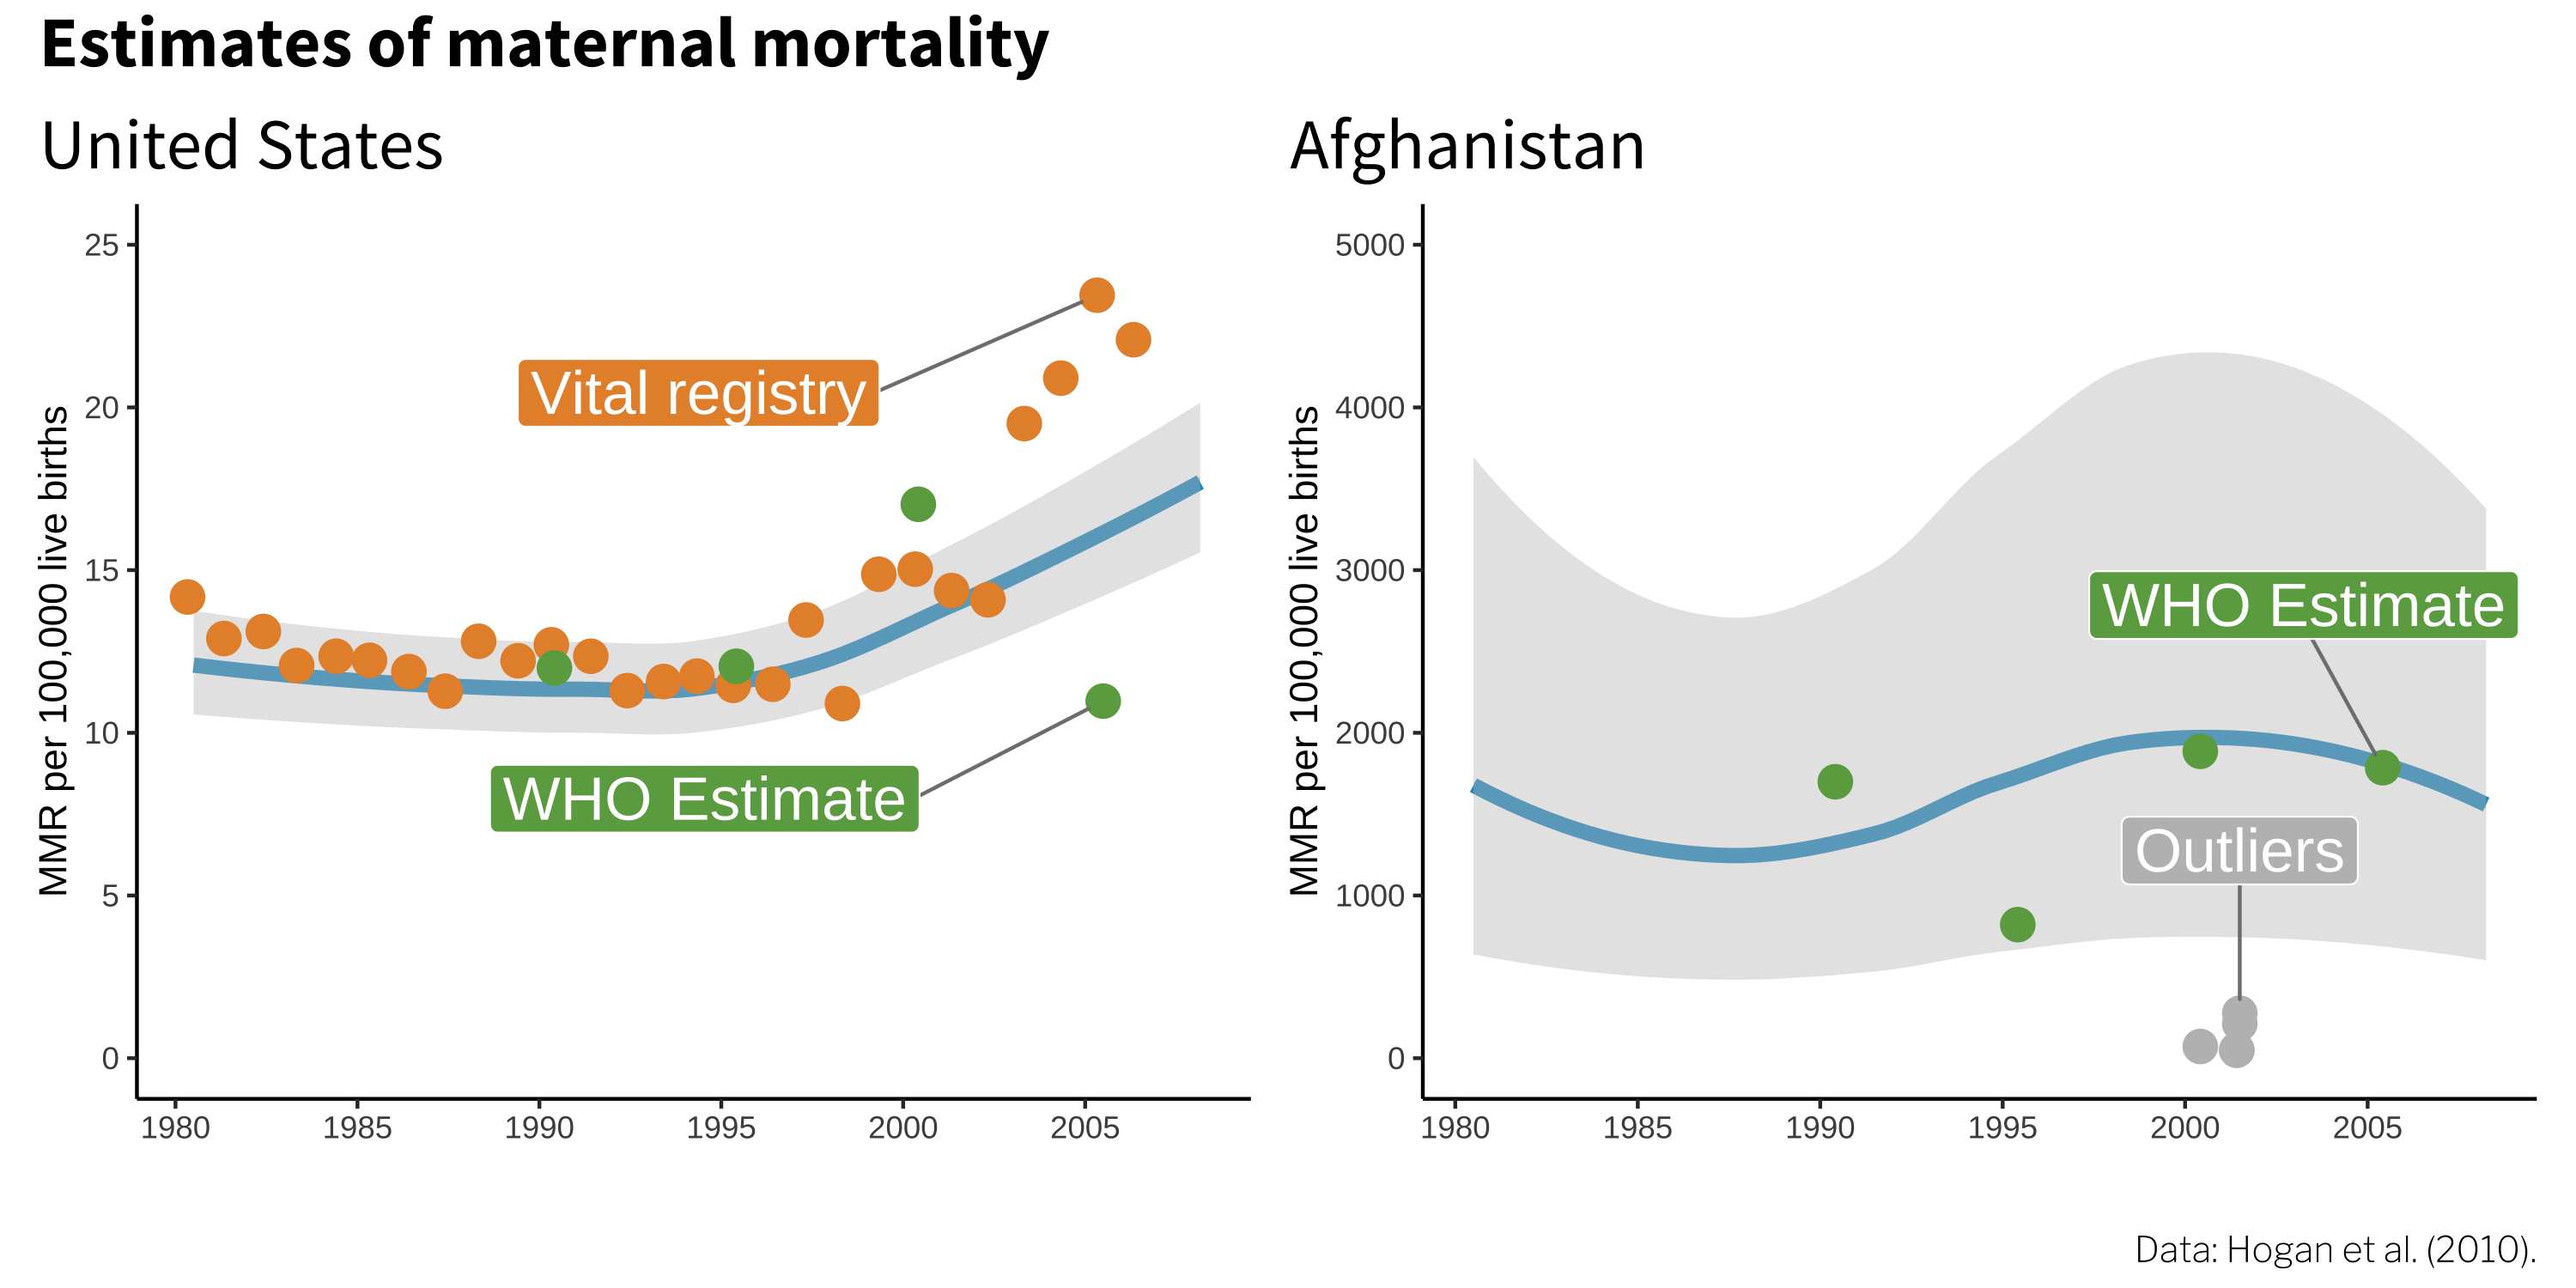
\includegraphics{images/figures/mmr.png}

}

\caption{\label{fig-mmr}Estimates of the maternal mortality rate in the
United States and Afghanistan.}

\end{figure*}

Now take a look at Afghanistan on the right. Note that the y-axis scale
is much larger in the 1000s, reflecting the fact that many more Afghan
women die of causes related to pregnancy or childbirth. Next, pay
attention to the width of the uncertainty band. It spans a range of more
than 3000 deaths. Compare this to a range of fewer than 5 deaths in the
US! This is because there are very few data points available to estimate
the `true' value in Afghanistan, and these individual data points can
differ by more than 1000 deaths.

The takeaway message is that there is uncertainty in everything. No
single estimate can be considered \emph{the} answer. Embrace uncertainty
and you will become a better scientist.

\hypertarget{what-constitutes-global-health-research}{%
\subsection{What Constitutes Global Health
Research?}\label{what-constitutes-global-health-research}}

Global health research brings together scholars and practitioners from
many different disciplines to tackle big challenges. Therefore, the
methods of these disciplines \emph{are} the methods of global health
research. We can organize the research landscape as shown in Figure
@ref(fig:basicapplied).

\begin{Shaded}
\begin{Highlighting}[]
\NormalTok{knitr}\SpecialCharTok{::}\FunctionTok{include\_graphics}\NormalTok{(}\StringTok{"images/basicapplied.pdf"}\NormalTok{, }\AttributeTok{dpi =} \ConstantTok{NA}\NormalTok{)}
\end{Highlighting}
\end{Shaded}

\begin{figure}[H]

{\centering 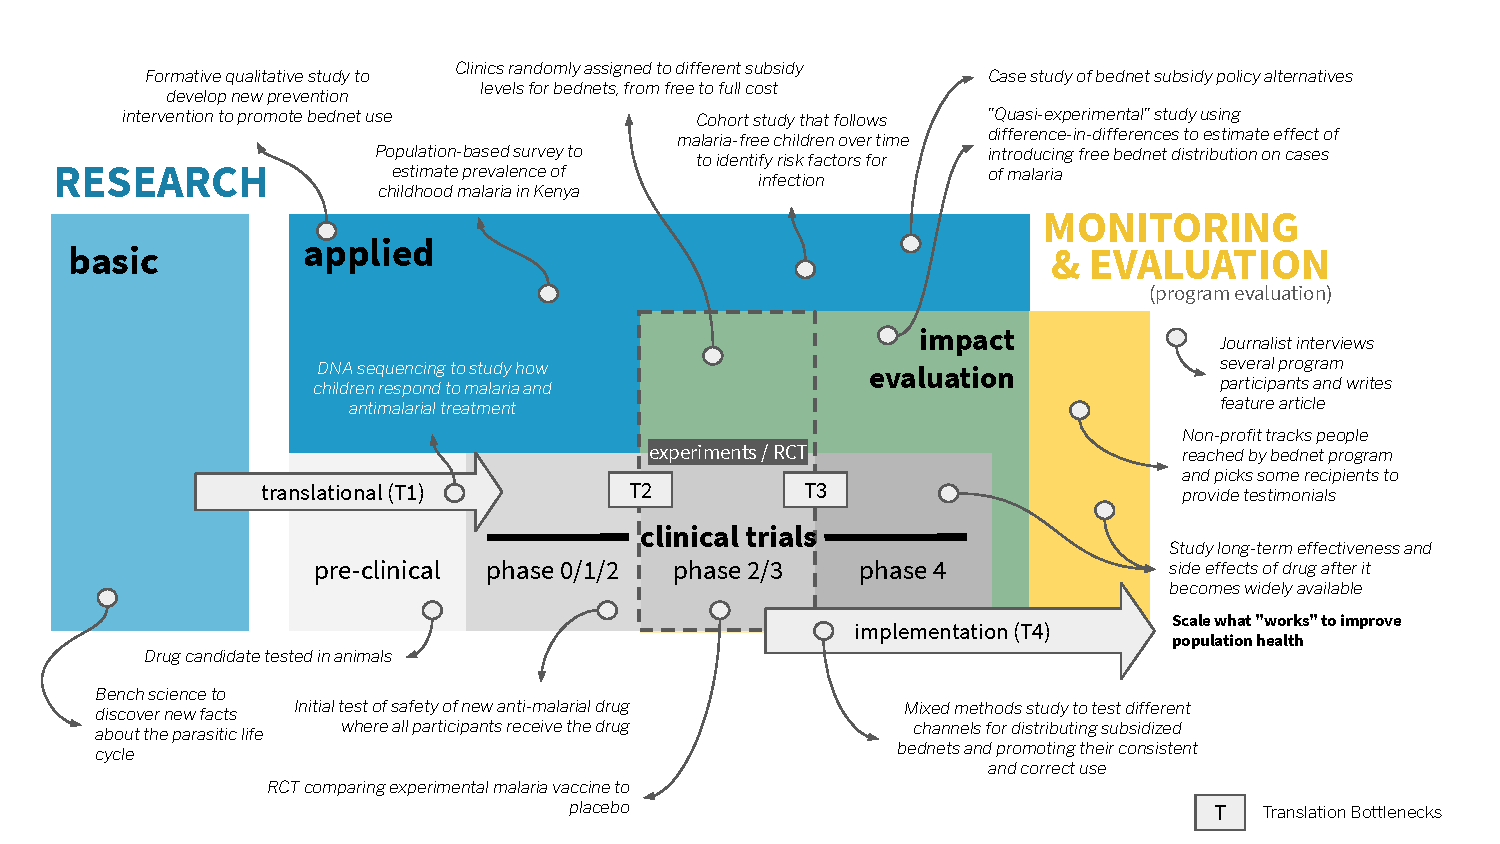
\includegraphics{images/basicapplied.pdf}

}

\caption{A research taxonomy}

\end{figure}

Research is divided into two main categories: basic and applied.
Overlapping with applied research is an area of work called ``monitoring
and evaluation'', or M\&E. Let's examine what constitutes research
before turning to M\&E.

\hypertarget{basic-research}{%
\subsubsection*{BASIC RESEARCH}\label{basic-research}}
\addcontentsline{toc}{subsubsection}{BASIC RESEARCH}

\begin{Shaded}
\begin{Highlighting}[]
\FunctionTok{cat}\NormalTok{(tufte}\SpecialCharTok{::}\FunctionTok{margin\_note}\NormalTok{(}\StringTok{"Basic research is sometimes referred to as the \textquotesingle{}bench\textquotesingle{} in the \textquotesingle{}bench to bedside\textquotesingle{} cascade of research needed to take an idea from the lab to a new medical treatment. This is accurate but incomplete. Fields like psychology also conduct basic research into constructs like emotion and violence that seek to expand our understanding. This is not \textquotesingle{}bench science\textquotesingle{} as typically imagined, but it\textquotesingle{}s basic research nonetheless."}\NormalTok{))}
\end{Highlighting}
\end{Shaded}

\marginnote{Basic research is sometimes referred to as the 'bench' in the 'bench to bedside' cascade of research needed to take an idea from the lab to a new medical treatment. This is accurate but incomplete. Fields like psychology also conduct basic research into constructs like emotion and violence that seek to expand our understanding. This is not 'bench science' as typically imagined, but it's basic research nonetheless.}

\textbf{Basic research}---also known as ``pure'' or ``blue skies''
research---is the pursuit of fundamental knowledge of phenomena. For
example, scientists conduct laboratory experiments to understand the
parasitic life cycle and how parasites interact with humans at different
stages. Another example is the scientific investigation of the
properties of cancer cells to better understand how they grow and
spread.

The information generated by basic science becomes the basis for applied
science. Harvard neurobiologist Dr.~Rachel Wilson explains this
beautifully:

\begin{Shaded}
\begin{Highlighting}[]
\FunctionTok{cat}\NormalTok{(tufte}\SpecialCharTok{::}\FunctionTok{margin\_note}\NormalTok{(}\StringTok{"}\SpecialCharTok{\textbackslash{}\textbackslash{}}\StringTok{faIcon\{youtube\} Scan the QR code to watch Dr. Wilson\textquotesingle{}s remarks at }\SpecialCharTok{\textbackslash{}\textbackslash{}}\StringTok{href\{http://ghr.link/fly\}\{}\SpecialCharTok{\textbackslash{}\textbackslash{}}\StringTok{footnotesize}\SpecialCharTok{\textbackslash{}\textbackslash{}}\StringTok{texttt\{ghr.link/fly\}\}."}\NormalTok{))}
\end{Highlighting}
\end{Shaded}

\marginnote{\faIcon{youtube} Scan the QR code to watch Dr. Wilson's remarks at \href{http://ghr.link/fly}{\footnotesize\texttt{ghr.link/fly}}.}

\begin{Shaded}
\begin{Highlighting}[]
\NormalTok{knitr}\SpecialCharTok{::}\FunctionTok{include\_graphics}\NormalTok{(}\StringTok{"images/QR\_fly.png"}\NormalTok{)}
\end{Highlighting}
\end{Shaded}

\begin{figure}[H]

{\centering 
\includegraphics[width=0.2\textwidth,height=\textheight]{images/QR_fly.png}

}

\end{figure}

\begin{Shaded}
\begin{Highlighting}[]
\FunctionTok{cat}\NormalTok{(tufte}\SpecialCharTok{::}\FunctionTok{margin\_note}\NormalTok{(}\StringTok{"\textless{}iframe width=\textquotesingle{}300\textquotesingle{} height=\textquotesingle{}169\textquotesingle{} src=\textquotesingle{}https://www.youtube.com/embed/uUnlPMeVusk\textquotesingle{} frameborder=\textquotesingle{}0\textquotesingle{} allow=\textquotesingle{}accelerometer; autoplay; encrypted{-}media; gyroscope; picture{-}in{-}picture\textquotesingle{} allowfullscreen\textgreater{}\textless{}/iframe\textgreater{}Watch Dr. Wilson\textquotesingle{}s full remarks."}\NormalTok{))}
\end{Highlighting}
\end{Shaded}

\begin{quote}
The new therapies of today were the prototypes of yesterday. And the
prototypes of yesterday were previously just findings in laboratories,
and before that they were just an idea. Unless we have new ideas, we're
not going to have useful therapies. Great new therapies don't just fall
like apples from a tree.
\end{quote}

\hypertarget{applied-research}{%
\subsubsection*{APPLIED RESEARCH}\label{applied-research}}
\addcontentsline{toc}{subsubsection}{APPLIED RESEARCH}

\textbf{Applied research} focuses on specific problems or real-world
applications. Much of global health research falls into the applied
domain because our mission is to improve health and achieve equity in
health for all people worldwide.

\hypertarget{clinical-research}{%
\paragraph*{Clinical Research}\label{clinical-research}}
\addcontentsline{toc}{paragraph}{Clinical Research}

Applied science takes many different forms, including clinical research.
\textbf{Clinical research} is a broad field that aims to understand
human disease, develop better ways to detect, diagnose, prevent, and
treat disease, and to promote health.{[}@roundtable:2002{]} Table
@ref(tab:clinical) lists several domains of clinical research.

\vspace{2em}

\begin{Shaded}
\begin{Highlighting}[]
\NormalTok{  clinical }\OtherTok{\textless{}{-}} \FunctionTok{tribble}\NormalTok{(}
    \SpecialCharTok{\textasciitilde{}}\NormalTok{Domain, }\SpecialCharTok{\textasciitilde{}}\NormalTok{Description,}
    \StringTok{"Treatment/prevention research"}\NormalTok{, }\StringTok{"Test new approaches for preventing or treating illness; includes clinical trials of drugs, biologics, devices, instruments, and behavioral interventions"}\NormalTok{,}
    \StringTok{"Screening research"}\NormalTok{, }\StringTok{"Develop and evaluate methods for detecting illness risk factors or markers"}\NormalTok{,}
    \StringTok{"Diagnostic research"}\NormalTok{, }\StringTok{"Develop and evaluate methods for identifying health conditions or illness"}\NormalTok{, }
    \StringTok{"Genetic studies"}\NormalTok{, }\StringTok{"Examine links between genes and disorders"}\NormalTok{, }
    \StringTok{"Epidemiological studies"}\NormalTok{, }\StringTok{"Study the patterns, causes, prevalence, and incidence of disease in a population"}\NormalTok{,}
    \StringTok{"Health services research"}\NormalTok{, }\StringTok{"Study how people access healthcare services, healthcare costs, and outcomes; operations research"}
\NormalTok{  )}
  
\NormalTok{format }\OtherTok{\textless{}{-}} \FunctionTok{ifelse}\NormalTok{(knitr}\SpecialCharTok{::}\FunctionTok{is\_html\_output}\NormalTok{(), }\StringTok{"html"}\NormalTok{, }\StringTok{"latex"}\NormalTok{)}

\FunctionTok{kable}\NormalTok{(clinical, }\AttributeTok{format =}\NormalTok{ format, }\AttributeTok{booktabs =}\NormalTok{ T,}
\AttributeTok{caption=}\StringTok{"Different types of clinical research"}\NormalTok{, }\AttributeTok{table.envir =} \StringTok{\textquotesingle{}table*\textquotesingle{}}\NormalTok{) }\SpecialCharTok{\%\textgreater{}\%}
  \FunctionTok{row\_spec}\NormalTok{(}\DecValTok{0}\NormalTok{, }\AttributeTok{bold=}\ConstantTok{TRUE}\NormalTok{) }\SpecialCharTok{\%\textgreater{}\%}
  \FunctionTok{column\_spec}\NormalTok{(}\DecValTok{1}\NormalTok{, }\AttributeTok{bold=}\ConstantTok{TRUE}\NormalTok{, }\AttributeTok{width=}\StringTok{"5cm"}\NormalTok{) }\SpecialCharTok{\%\textgreater{}\%}
  \FunctionTok{column\_spec}\NormalTok{(}\DecValTok{2}\NormalTok{, }\AttributeTok{width=}\StringTok{"10.5cm"}\NormalTok{) }\SpecialCharTok{\%\textgreater{}\%}
    \FunctionTok{kable\_styling}\NormalTok{(}\AttributeTok{full\_width =}\NormalTok{ F, }\AttributeTok{position =} \StringTok{"left"}\NormalTok{)}
\end{Highlighting}
\end{Shaded}

\begin{table*}

\caption{Different types of clinical research}
\begin{tabular}[t]{>{\raggedright\arraybackslash}p{5cm}>{\raggedright\arraybackslash}p{10.5cm}}
\toprule
\textbf{Domain} & \textbf{Description}\\
\midrule
\textbf{Treatment/prevention research} & Test new approaches for preventing or treating illness; includes clinical trials of drugs, biologics, devices, instruments, and behavioral interventions\\
\textbf{Screening research} & Develop and evaluate methods for detecting illness risk factors or markers\\
\textbf{Diagnostic research} & Develop and evaluate methods for identifying health conditions or illness\\
\textbf{Genetic studies} & Examine links between genes and disorders\\
\textbf{Epidemiological studies} & Study the patterns, causes, prevalence, and incidence of disease in a population\\
\addlinespace
\textbf{Health services research} & Study how people access healthcare services, healthcare costs, and outcomes; operations research\\
\bottomrule
\end{tabular}
\end{table*}

\vspace{2em}

\newpage

\begin{Shaded}
\begin{Highlighting}[]
\FunctionTok{cat}\NormalTok{(tufte}\SpecialCharTok{::}\FunctionTok{margin\_note}\NormalTok{(}\StringTok{"}\SpecialCharTok{\textbackslash{}\textbackslash{}}\StringTok{faIcon\{youtube\} These phases are broadly similar across different regulatory bodies around the world, including the U.S. Federal Drug Administration (FDA), the European Medicines Agency (EMA), the Central Drugs Standard Control Organization in India, and the National Medical Products Administration in China, among many others. Scan the QR code to watch a brief overview of the phases from the NIH\textquotesingle{}s National Cancer Institute, }\SpecialCharTok{\textbackslash{}\textbackslash{}}\StringTok{href\{https://ghr.link/fda\}\{}\SpecialCharTok{\textbackslash{}\textbackslash{}}\StringTok{footnotesize}\SpecialCharTok{\textbackslash{}\textbackslash{}}\StringTok{texttt\{ghr.link/fda\}\}.}\SpecialCharTok{\textbackslash{}\textbackslash{}}\StringTok{vspace\{0cm\}"}\NormalTok{))}
\end{Highlighting}
\end{Shaded}

\marginnote{\faIcon{youtube} These phases are broadly similar across different regulatory bodies around the world, including the U.S. Federal Drug Administration (FDA), the European Medicines Agency (EMA), the Central Drugs Standard Control Organization in India, and the National Medical Products Administration in China, among many others. Scan the QR code to watch a brief overview of the phases from the NIH's National Cancer Institute, \href{https://ghr.link/fda}{\footnotesize\texttt{ghr.link/fda}}.\vspace{0cm}}

\begin{Shaded}
\begin{Highlighting}[]
\NormalTok{knitr}\SpecialCharTok{::}\FunctionTok{include\_graphics}\NormalTok{(}\StringTok{"images/QR\_fda.png"}\NormalTok{)}
\end{Highlighting}
\end{Shaded}

\begin{figure}[H]

{\centering 
\includegraphics[width=0.2\textwidth,height=\textheight]{images/QR_fda.png}

}

\end{figure}

\begin{Shaded}
\begin{Highlighting}[]
\FunctionTok{cat}\NormalTok{(tufte}\SpecialCharTok{::}\FunctionTok{margin\_note}\NormalTok{(}\StringTok{"\textless{}iframe width=\textquotesingle{}300\textquotesingle{} height=\textquotesingle{}169\textquotesingle{} src=\textquotesingle{}https://www.youtube.com/embed/dsfPOpE{-}GEs\textquotesingle{} frameborder=\textquotesingle{}0\textquotesingle{} allow=\textquotesingle{}accelerometer; autoplay; encrypted{-}media; gyroscope; picture{-}in{-}picture\textquotesingle{} allowfullscreen\textgreater{}\textless{}/iframe\textgreater{}These phases are broadly similar across different regulatory bodies around the world, including the U.S. Federal Drug Administration (FDA), the European Medicines Agency (EMA), the Central Drugs Standard Control Organization in India, and the National Medical Products Administration in China, among many others. Here\textquotesingle{}s a brief overview of the phases from the NIH\textquotesingle{}s National Cancer Institute."}\NormalTok{))}
\end{Highlighting}
\end{Shaded}

One type of clinical research is a clinical trial. Table
@ref(tab:phases) lists the phases of trials that drugs, biologics,
devices, and instruments complete prior to going to market. In the early
phases of drug trials, the objective is to understand how the compound
affects the body. What is a safe dose that could be effective? Phase 3
trials put the optimal dose to the test, seeking to determine if the
drug ``works'' and to quantify the size of the effect. Drugs that pass
this test are typically approved for use by the governing regulatory
body. Once a drug reaches market, Phase 4 trials monitor side effects
and efficacy over time.

\vspace{1em}

\begin{Shaded}
\begin{Highlighting}[]
\NormalTok{phases }\OtherTok{\textless{}{-}} \FunctionTok{tribble}\NormalTok{(}
    \SpecialCharTok{\textasciitilde{}}\StringTok{"Phase"}\NormalTok{, }\SpecialCharTok{\textasciitilde{}}\StringTok{"Enrollment"}\NormalTok{, }\SpecialCharTok{\textasciitilde{}}\StringTok{"Goal"}\NormalTok{,}
  \StringTok{"Preclinical research"}\NormalTok{, }\StringTok{""}\NormalTok{, }\StringTok{"Are there signs that the drug candidate will have an effect in the lab?"}\NormalTok{,}
  \StringTok{"0"}\NormalTok{, }\StringTok{"\textless{}10"}\NormalTok{, }\StringTok{"What happens in the body (pharmacokinetics) when a very low dose is administered to human subjects? (optional phase)"}\NormalTok{,}
  \StringTok{"1"}\NormalTok{, }\StringTok{"10s"}\NormalTok{, }\StringTok{"Is the drug safe? What is the best dose that balances possible effects with toxicity?"}\NormalTok{,}
  \StringTok{"2"}\NormalTok{, }\StringTok{"100s"}\NormalTok{, }\StringTok{"When using this optimal dose, is there any effect of the drug on clinical markers or health outcomes?"}\NormalTok{,}
  \StringTok{"3"}\NormalTok{, }\StringTok{"1000s"}\NormalTok{, }\StringTok{"What is the effect of the drug on clinical markers or health outcomes when compared to an existing treatment or placebo in a randomized evaluation? Success at this stage is required for regulatory approval in some countries."}\NormalTok{,}
  \StringTok{"4"}\NormalTok{, }\StringTok{""}\NormalTok{, }\StringTok{"Are there long{-}term adverse effects of the drug once it is available on the market?"}
\NormalTok{)  }
  
\NormalTok{format }\OtherTok{\textless{}{-}} \FunctionTok{ifelse}\NormalTok{(knitr}\SpecialCharTok{::}\FunctionTok{is\_html\_output}\NormalTok{(), }\StringTok{"html"}\NormalTok{, }\StringTok{"latex"}\NormalTok{)}

\FunctionTok{kable}\NormalTok{(phases, }\AttributeTok{format =}\NormalTok{ format, }\AttributeTok{booktabs =}\NormalTok{ T,}
\AttributeTok{caption=}\StringTok{"Clinical trial phases"}\NormalTok{, }\AttributeTok{table.envir =} \StringTok{\textquotesingle{}table*\textquotesingle{}}\NormalTok{) }\SpecialCharTok{\%\textgreater{}\%}
  \FunctionTok{row\_spec}\NormalTok{(}\DecValTok{0}\NormalTok{, }\AttributeTok{bold=}\ConstantTok{TRUE}\NormalTok{) }\SpecialCharTok{\%\textgreater{}\%}
  \FunctionTok{column\_spec}\NormalTok{(}\DecValTok{1}\NormalTok{, }\AttributeTok{bold=}\ConstantTok{TRUE}\NormalTok{, }\AttributeTok{width=}\StringTok{"3.5cm"}\NormalTok{) }\SpecialCharTok{\%\textgreater{}\%}
  \FunctionTok{column\_spec}\NormalTok{(}\DecValTok{3}\NormalTok{, }\AttributeTok{width=}\StringTok{"10cm"}\NormalTok{) }\SpecialCharTok{\%\textgreater{}\%}  
    \FunctionTok{kable\_styling}\NormalTok{(}\AttributeTok{full\_width =}\NormalTok{ F, }\AttributeTok{position =} \StringTok{"left"}\NormalTok{)}
\end{Highlighting}
\end{Shaded}

\begin{table*}

\caption{Clinical trial phases}
\begin{tabular}[t]{>{\raggedright\arraybackslash}p{3.5cm}l>{\raggedright\arraybackslash}p{10cm}}
\toprule
\textbf{Phase} & \textbf{Enrollment} & \textbf{Goal}\\
\midrule
\textbf{Preclinical research} &  & Are there signs that the drug candidate will have an effect in the lab?\\
\textbf{0} & <10 & What happens in the body (pharmacokinetics) when a very low dose is administered to human subjects? (optional phase)\\
\textbf{1} & 10s & Is the drug safe? What is the best dose that balances possible effects with toxicity?\\
\textbf{2} & 100s & When using this optimal dose, is there any effect of the drug on clinical markers or health outcomes?\\
\textbf{3} & 1000s & What is the effect of the drug on clinical markers or health outcomes when compared to an existing treatment or placebo in a randomized evaluation? Success at this stage is required for regulatory approval in some countries.\\
\addlinespace
\textbf{4} &  & Are there long-term adverse effects of the drug once it is available on the market?\\
\bottomrule
\end{tabular}
\end{table*}

\vspace{2em}

\begin{Shaded}
\begin{Highlighting}[]
\FunctionTok{cat}\NormalTok{(tufte}\SpecialCharTok{::}\FunctionTok{margin\_note}\NormalTok{(}\StringTok{"}\SpecialCharTok{\textbackslash{}\textbackslash{}}\StringTok{faIcon\{book{-}reader\} Scan the QR code to to see a list of international trial registries, }\SpecialCharTok{\textbackslash{}\textbackslash{}}\StringTok{href\{http://ghr.link/ask\}\{}\SpecialCharTok{\textbackslash{}\textbackslash{}}\StringTok{footnotesize}\SpecialCharTok{\textbackslash{}\textbackslash{}}\StringTok{texttt\{ghr.link/ask\}\}."}\NormalTok{))}
\end{Highlighting}
\end{Shaded}

\marginnote{\faIcon{book-reader} Scan the QR code to to see a list of international trial registries, \href{http://ghr.link/ask}{\footnotesize\texttt{ghr.link/ask}}.}

\begin{Shaded}
\begin{Highlighting}[]
\NormalTok{knitr}\SpecialCharTok{::}\FunctionTok{include\_graphics}\NormalTok{(}\StringTok{"images/QR\_ask.png"}\NormalTok{)}
\end{Highlighting}
\end{Shaded}

\begin{figure}[H]

{\centering 
\includegraphics[width=0.2\textwidth,height=\textheight]{images/QR_ask.png}

}

\end{figure}

\begin{Shaded}
\begin{Highlighting}[]
\FunctionTok{cat}\NormalTok{(tufte}\SpecialCharTok{::}\FunctionTok{margin\_note}\NormalTok{(}\StringTok{"Click [here](http://ghr.link/ask) to see a list of international trial registries."}\NormalTok{))}
\end{Highlighting}
\end{Shaded}

In the United States, the FDA requires that most interventional studies
of any regulated products with research sites in the U.S. be registered
in the \emph{ClinicalTrials.gov} trial registry.{[}@fda:2007{]} Many
countries have their own registries, and the World Health Organization
maintains a web portal that searches across registries.

\begin{Shaded}
\begin{Highlighting}[]
\FunctionTok{cat}\NormalTok{(tufte}\SpecialCharTok{::}\FunctionTok{margin\_note}\NormalTok{(}\StringTok{"}\SpecialCharTok{\textbackslash{}\textbackslash{}}\StringTok{faIcon\{book{-}reader\} Scan the QR code to read about Aunt Debbie\textquotesingle{}s experience in a Phase 1 poliovirus trial at Duke University, }\SpecialCharTok{\textbackslash{}\textbackslash{}}\StringTok{href\{http://ghr.link/van\}\{}\SpecialCharTok{\textbackslash{}\textbackslash{}}\StringTok{footnotesize}\SpecialCharTok{\textbackslash{}\textbackslash{}}\StringTok{texttt\{ghr.link/van\}\}."}\NormalTok{))}
\end{Highlighting}
\end{Shaded}

\marginnote{\faIcon{book-reader} Scan the QR code to read about Aunt Debbie's experience in a Phase 1 poliovirus trial at Duke University, \href{http://ghr.link/van}{\footnotesize\texttt{ghr.link/van}}.}

\begin{Shaded}
\begin{Highlighting}[]
\NormalTok{knitr}\SpecialCharTok{::}\FunctionTok{include\_graphics}\NormalTok{(}\StringTok{"images/QR\_van.png"}\NormalTok{)}
\end{Highlighting}
\end{Shaded}

\begin{figure}[H]

{\centering 
\includegraphics[width=0.2\textwidth,height=\textheight]{images/QR_van.png}

}

\end{figure}

\begin{Shaded}
\begin{Highlighting}[]
\FunctionTok{cat}\NormalTok{(tufte}\SpecialCharTok{::}\FunctionTok{margin\_note}\NormalTok{(}\StringTok{"Click [here](http://ghr.link/van) to read about Aunt Debbie\textquotesingle{}s experience in a Phase 1 poliovirus trial at Duke University."}\NormalTok{))}
\end{Highlighting}
\end{Shaded}

Trial registries are useful for researchers and patients alike. When my
wife's Aunt Debbie learned she had an aggressive brain tumor, we
searched \emph{ClinicalTrials.gov} and identified several trials
recruiting patients for experimental glioblastoma treatments. Debbie
decided to take part in a Phase 1 trial that injected modified
poliovirus into her tumor. She lived for another five years and helped
to advance the science of glioblastoma treatment.

Healthy volunteers and patients like Debbie are the backbone of clinical
research. Their sacrifices, combined with the ingenuity of scientists
and research teams, have created thousands of medical breakthroughs. But
for every new drug approved, there is a trail of failure (see Figure
@ref(fig:ctrial)). Recent studies estimate that fewer than 15\% of
candidates entering Phase 1 trials are ultimately approved by the FDA
{[}@wong:2019{]}.

\begin{Shaded}
\begin{Highlighting}[]
\NormalTok{knitr}\SpecialCharTok{::}\FunctionTok{include\_graphics}\NormalTok{(here}\SpecialCharTok{::}\FunctionTok{here}\NormalTok{(}\StringTok{"images"}\NormalTok{, }\StringTok{"figures"}\NormalTok{, }\FunctionTok{paste0}\NormalTok{(opts\_current}\SpecialCharTok{$}\FunctionTok{get}\NormalTok{(}\StringTok{"label"}\NormalTok{), }\StringTok{".png"}\NormalTok{))) }
\end{Highlighting}
\end{Shaded}

\begin{figure}[H]

{\centering 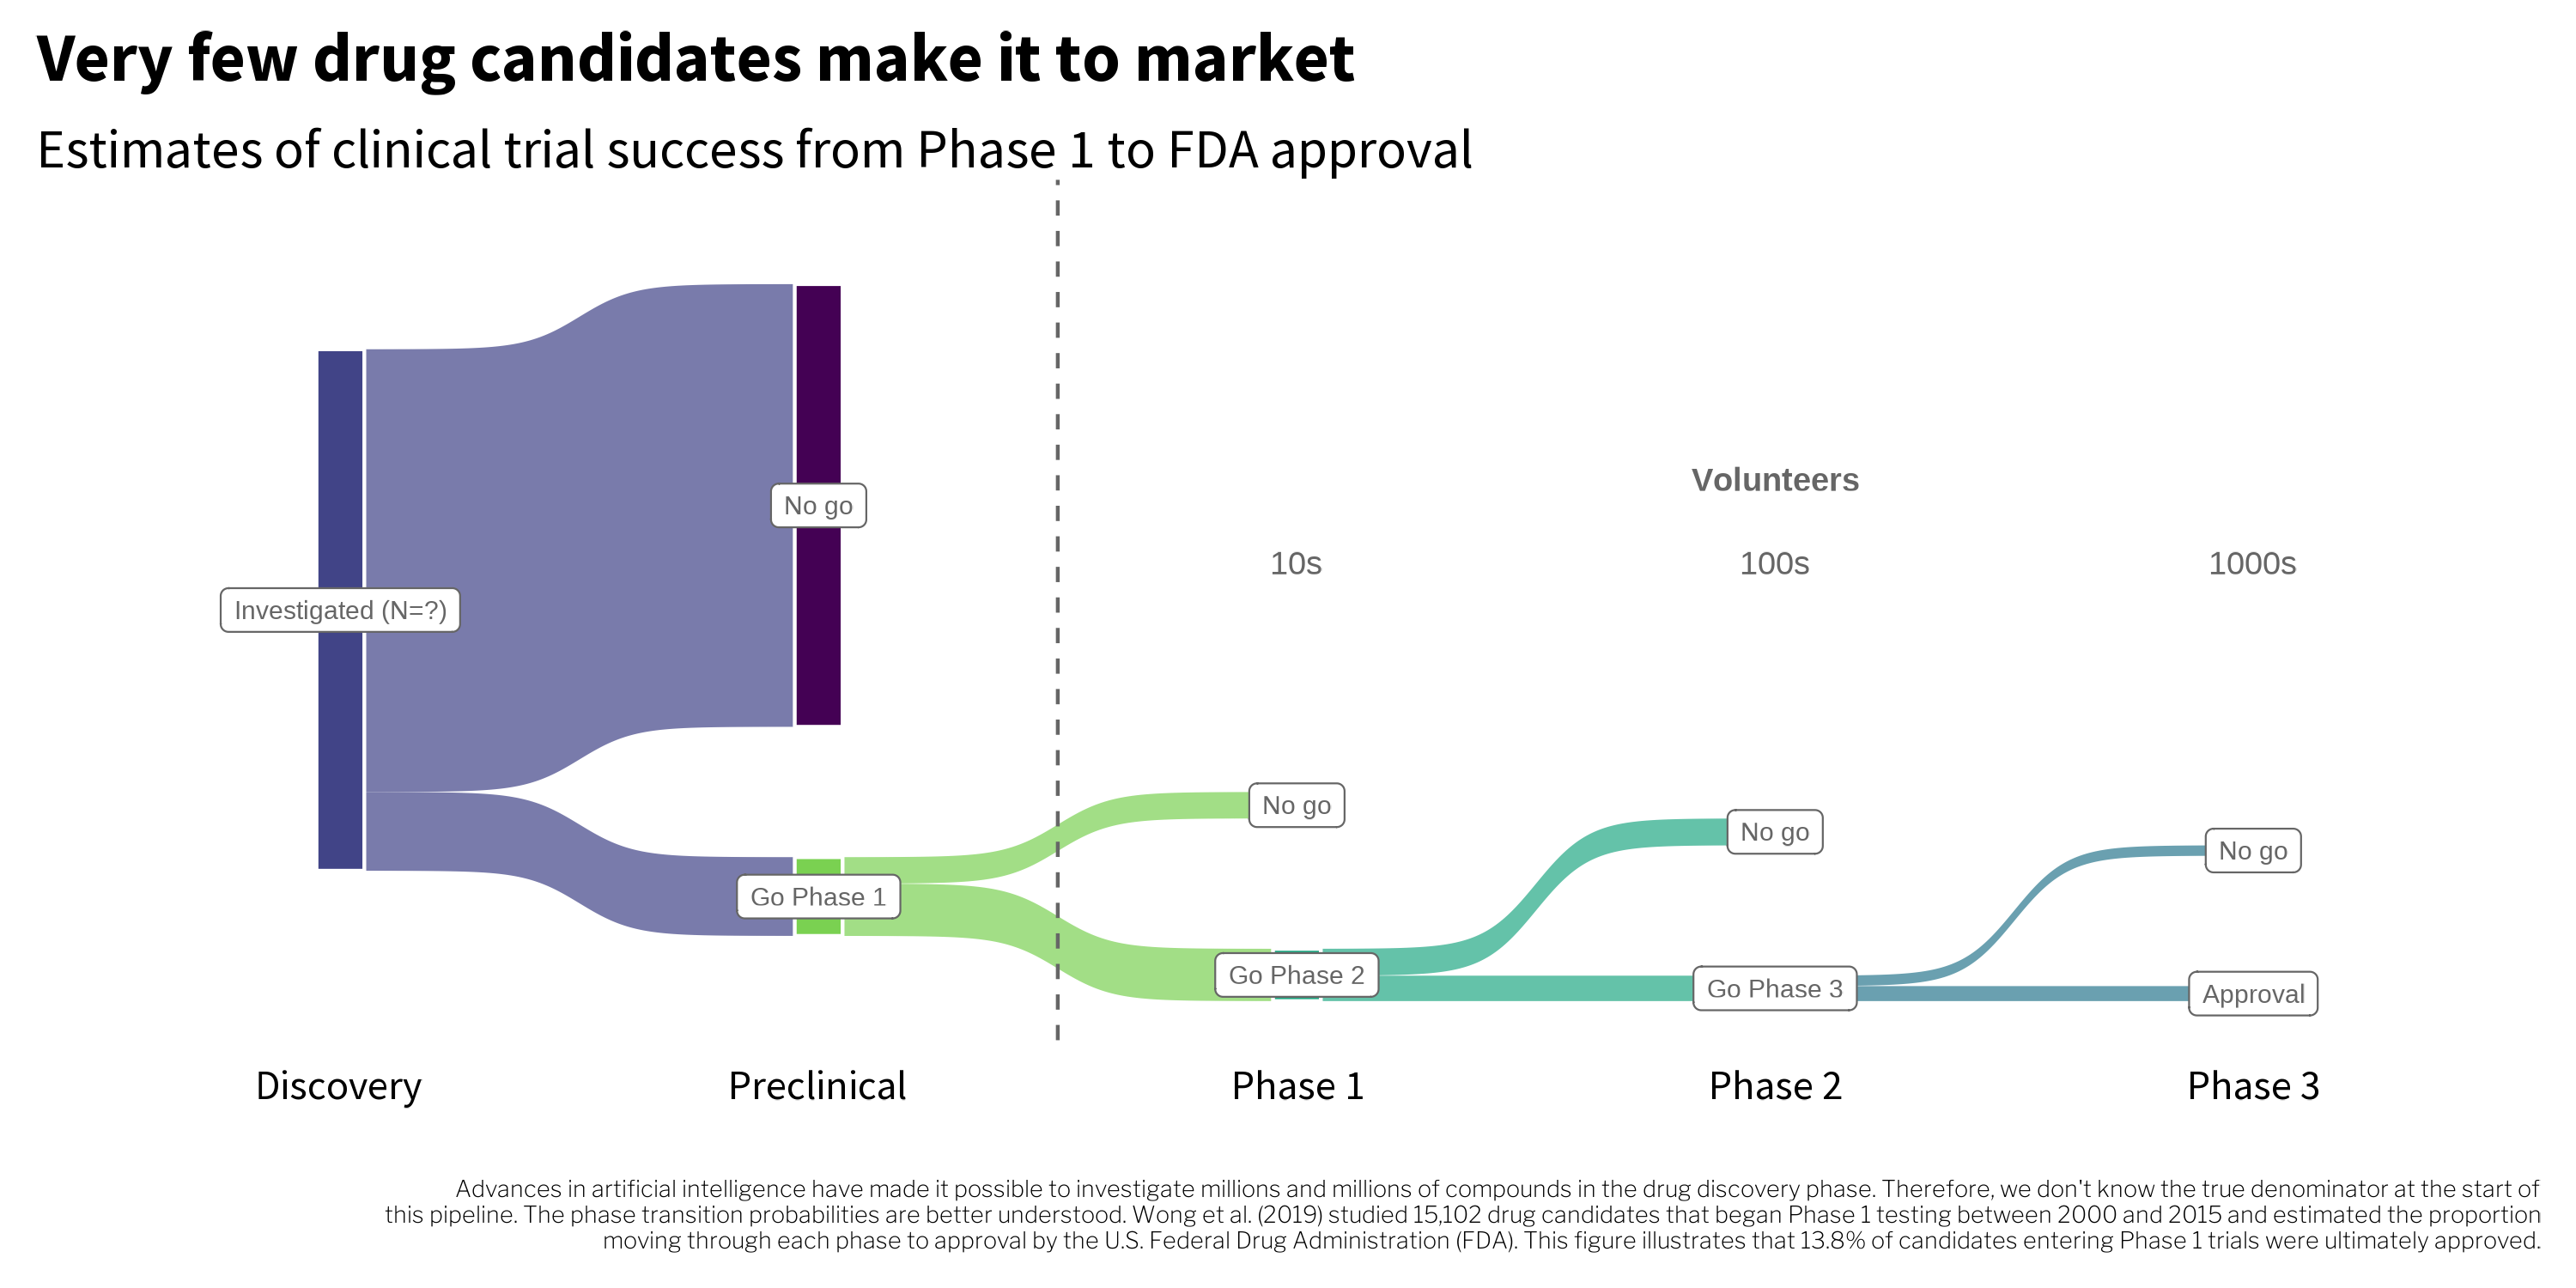
\includegraphics[width=1\textwidth,height=\textheight]{/Users/epg4/Dropbox (Personal)/repos/ghr_book/images/figures/ctrial.png}

}

\caption{Pipeline from basic research to FDA approval.}

\end{figure}

This pipeline does not include studies of behavioral interventions,
social programs, or policies because the FDA only regulates drugs,
biologics, devices, and instruments. Nevertheless, we still design
studies to estimate the efficacy of interventions, programs, and
policies, and many of these tests meet the World Health Organization's
definition of a `clinical trial':{[}@who:clinical{]}

\begin{Shaded}
\begin{Highlighting}[]
\FunctionTok{cat}\NormalTok{(tufte}\SpecialCharTok{::}\FunctionTok{margin\_note}\NormalTok{(}\StringTok{"The International Committee of Medical Journal Editors adopted this definition in 2007 and recommended that all clinical trials should be registered in an appropriate trial registry. Many peer{-}reviewed health journals follow this guidance and will not accept manuscripts from unregistered studies."}\NormalTok{))}
\end{Highlighting}
\end{Shaded}

\marginnote{The International Committee of Medical Journal Editors adopted this definition in 2007 and recommended that all clinical trials should be registered in an appropriate trial registry. Many peer-reviewed health journals follow this guidance and will not accept manuscripts from unregistered studies.}

\begin{quote}
any research study that prospectively assigns human participants or
groups of humans to one or more health-related interventions to evaluate
the effects on health outcomes. (World Health Organization definition)
\end{quote}

\newpage

\vspace{2cm}

\begin{Shaded}
\begin{Highlighting}[]
\FunctionTok{cat}\NormalTok{(tufte}\SpecialCharTok{::}\FunctionTok{margin\_note}\NormalTok{(}\StringTok{"}\SpecialCharTok{\textbackslash{}\textbackslash{}}\StringTok{faIcon\{youtube\} Scan the QR code to watch Dr. Pedro Alonso from the World Health Organization explain why this vaccine is a breakthrough in the prevention of malaria, }\SpecialCharTok{\textbackslash{}\textbackslash{}}\StringTok{href\{https://ghr.link/vax\}\{}\SpecialCharTok{\textbackslash{}\textbackslash{}}\StringTok{footnotesize}\SpecialCharTok{\textbackslash{}\textbackslash{}}\StringTok{texttt\{ghr.link/vax\}\}.}\SpecialCharTok{\textbackslash{}\textbackslash{}}\StringTok{vspace\{0cm\}"}\NormalTok{))}
\end{Highlighting}
\end{Shaded}

\marginnote{\faIcon{youtube} Scan the QR code to watch Dr. Pedro Alonso from the World Health Organization explain why this vaccine is a breakthrough in the prevention of malaria, \href{https://ghr.link/vax}{\footnotesize\texttt{ghr.link/vax}}.\vspace{0cm}}

\begin{Shaded}
\begin{Highlighting}[]
\NormalTok{knitr}\SpecialCharTok{::}\FunctionTok{include\_graphics}\NormalTok{(}\StringTok{"images/QR\_vax.png"}\NormalTok{)}
\end{Highlighting}
\end{Shaded}

\begin{figure}[H]

{\centering 
\includegraphics[width=0.2\textwidth,height=\textheight]{images/QR_vax.png}

}

\end{figure}

\begin{Shaded}
\begin{Highlighting}[]
\FunctionTok{cat}\NormalTok{(tufte}\SpecialCharTok{::}\FunctionTok{margin\_note}\NormalTok{(}\StringTok{"\textless{}iframe width=\textquotesingle{}300\textquotesingle{} height=\textquotesingle{}169\textquotesingle{} src=\textquotesingle{}https://www.youtube.com/embed/U2V6R2YC22s\textquotesingle{} title=\textquotesingle{}YouTube video player\textquotesingle{} frameborder=\textquotesingle{}0\textquotesingle{} allow=\textquotesingle{}accelerometer; autoplay; clipboard{-}write; encrypted{-}media; gyroscope; picture{-}in{-}picture\textquotesingle{} allowfullscreen\textgreater{}\textless{}/iframe\textgreater{}Dr. Pedro Alonso from the World Health Organization explains why this vaccine is a breakthrough in the prevention of malaria."}\NormalTok{))}
\end{Highlighting}
\end{Shaded}

\begin{blackbox}

\begin{center}
\textbf{CASE STUDY: Developing the first malaria vaccine}

\end{center}

\vspace{.2cm}

In 2021, after more than 35 years of research, the World Health
Organization recommended widespread use of a vaccine candidate called
RTS,S/AS01, or Mosquirix™, to prevent \emph{P. falciparum} malaria in
children.

\vspace{.2cm}

Development of RTS,S/AS01 began in 1984, and soon after, a promising
vaccine candidate entered preclinical research. Researchers performed
tests on nonhuman subjects to collect data on how well the vaccine
worked (efficacy), how much damage it could do to an organism
(toxicity), and how the body affected the vaccine (pharmacokinetics).

\vspace{.2cm}

Clinical research on humans began in 1992. Researchers conducted a Phase
1 safety and immunogenicity trial with 20 adults in The Gambia in 1997.
Results suggested that the vaccine did not have any significant toxicity
but did produce the expected antibodies.

\vspace{.2cm}

Several Phase 2 studies conducted over the next decade demonstrated the
efficacy of the vaccine against several endpoints. A Phase 2b trial
began in Mozambique in 2003 with more than 2,000 children. Each child
was randomly assigned to receive 3 doses of RTS,S or a control vaccine.
After 6 months, the prevalence of malaria was 37\% lower in the
treatment group than in the control group. This Phase 2 trial was an
important proof-of-concept study.

\vspace{.2cm}

The results of a large Phase 3 trial with more than 15,000 infants and
young children in 7 African countries were published in 2015. Children
who participated in the study were randomly assigned to 1 of 3 arms: (i)
3 doses of RTS,S and a booster dose at month 20, (ii) 3 doses of RTS,S
and a booster dose of a comparator vaccine at month 20, or (iii) 4 doses
of a comparator vaccine. RTS,S reduced clinical malaria cases by 28\%
and 18\% among young children and infants, respectively, over a 3 to
4-year period. This Phase 3 trial demonstrated that the treatment was
efficacious.

\vspace{.2cm}

On the basis of these results, the European Medicines Agency issued a
favorable ``European scientific opinion''. This led the health
ministries in Ghana, Kenya and Malawi to authorize a pilot study in 2019
to assess the feasibility of administering the required four doses of
the vaccine as part of routine childhood immunization programs. After
more than 800,000 children were immunized under this program, the WHO
recommended that countries with moderate to high transmission adopt the
vaccine.

\end{blackbox}

\hypertarget{translational-implementation-and-policy-research}{%
\paragraph*{Translational, Implementation, and Policy
Research}\label{translational-implementation-and-policy-research}}
\addcontentsline{toc}{paragraph}{Translational, Implementation, and
Policy Research}

\begin{Shaded}
\begin{Highlighting}[]
\FunctionTok{cat}\NormalTok{(tufte}\SpecialCharTok{::}\FunctionTok{margin\_note}\NormalTok{(}\StringTok{"Bauer and Kirchner make the point that our failure to put good ideas to use is not a new phenonmenon. The British Navy observed in 1601 that citrus cured scurvy on long sea voyages—and collected confirming \textquotesingle{}trial\textquotesingle{} evidence in 1747—but it was not until 1795 that using citrus became routine practice."}\NormalTok{))}
\end{Highlighting}
\end{Shaded}

\marginnote{Bauer and Kirchner make the point that our failure to put good ideas to use is not a new phenonmenon. The British Navy observed in 1601 that citrus cured scurvy on long sea voyages—and collected confirming 'trial' evidence in 1747—but it was not until 1795 that using citrus became routine practice.}

It's a long road from idea to impact,{[}@morris:2011{]} and most ideas
don't complete the trip.{[}@bauer:2020{]} Practitioners of
\textbf{translational research} point to four key bottlenecks where
ideas often stall (see also Figure @ref(fig:basicapplied)):

\begin{itemize}
\tightlist
\item
  T1: Translation from basic science to clinical research
\item
  T2: Translation from early clinical trials to Phase 3 trials and
  beyond with larger patient populations
\item
  T3: Translation from efficacy trials (i.e., Phase 3 trials) to
  real-world effectiveness through implementation research
\item
  T4: Translation from evidence about delivery at scale to the adoption
  of new policies
\end{itemize}

Translational research originally focused on moving from ``bench to
bedside'', or from basic research in the lab to clinical research with
humans (T1), and later expanded to address the challenge of moving from
early to late-stage human trials (T2). Today we recognize that other
bottlenecks (T3 and T4) prevent good ideas from impacting population
health and policy.{[}@woolf:2008{]}

For instance, we know that giving children a simple mixture of water,
sugar, and salts when they are dehydrated from diarrhea can prevent
death in 90\% of cases, but only 4 in 10 children receive this life
saving oral rehydration therapy (ORT).{[}@dadonaite:2019{]} And each
year, several hundred thousand children under five years die from
diarrheal diseases.

\begin{Shaded}
\begin{Highlighting}[]
\NormalTok{knitr}\SpecialCharTok{::}\FunctionTok{include\_graphics}\NormalTok{(}\StringTok{"images/AR2017\_Delivery\_Challenge.jpg"}\NormalTok{, }\AttributeTok{dpi =} \ConstantTok{NA}\NormalTok{)}
\end{Highlighting}
\end{Shaded}

\begin{Shaded}
\begin{Highlighting}[]
\NormalTok{knitr}\SpecialCharTok{::}\FunctionTok{include\_graphics}\NormalTok{(}\StringTok{"images/AR2017\_Delivery\_Challenge.pdf"}\NormalTok{, }\AttributeTok{dpi =} \ConstantTok{NA}\NormalTok{)}
\end{Highlighting}
\end{Shaded}

\begin{figure}[H]

{\centering 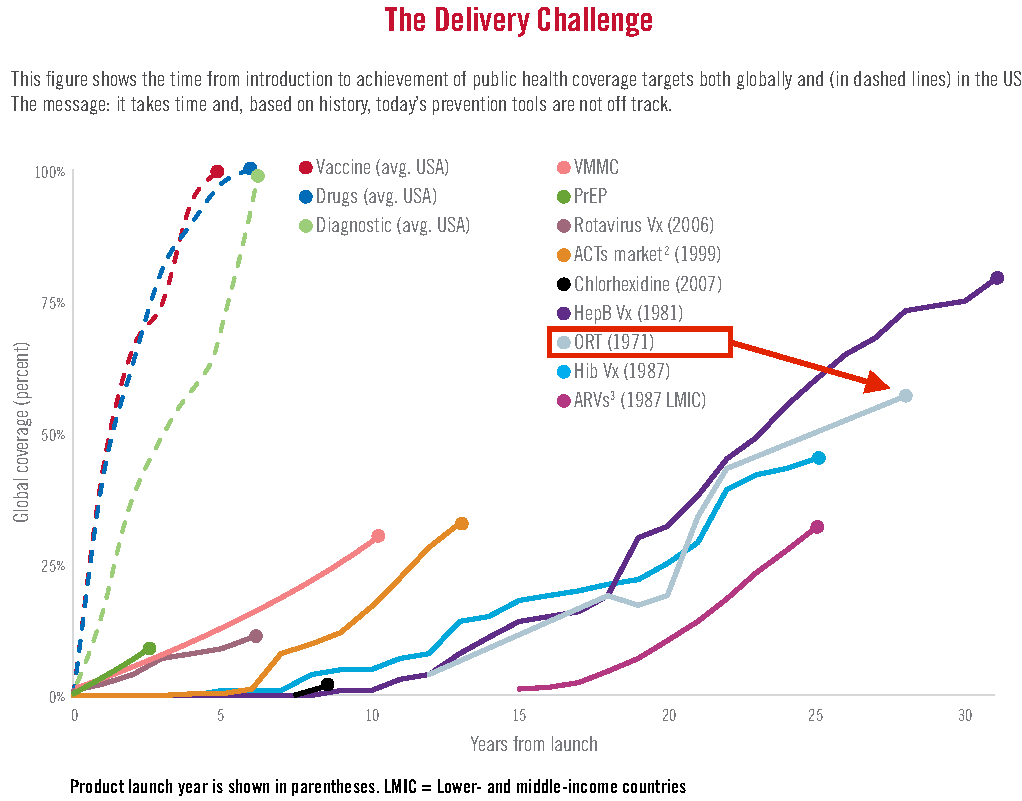
\includegraphics{images/AR2017_Delivery_Challenge.pdf}

}

\caption{Time from introduction to achievement of public health coverage
targets. Source: AVAC Report 2017: Mixed Messages and How to Untangle
Them. avac.org/report2017}

\end{figure}

This is an example of a `delivery gap' or `know-do' gap in global
health---the space between discovering what works and delivering the
solution at scale (see Figure @ref(fig:timetocoveragelatex) for other
examples).

\newpage

\begin{Shaded}
\begin{Highlighting}[]
\FunctionTok{cat}\NormalTok{(tufte}\SpecialCharTok{::}\FunctionTok{margin\_note}\NormalTok{(}\StringTok{"Work in this area has evolved independently across several disciplines. In addition to translational research and implementation research, you can find references to dissemination science, diffusion of innovations, quality improvement, knowledge transfer, and learning healthcare systems."}\NormalTok{))}
\end{Highlighting}
\end{Shaded}

\marginnote{Work in this area has evolved independently across several disciplines. In addition to translational research and implementation research, you can find references to dissemination science, diffusion of innovations, quality improvement, knowledge transfer, and learning healthcare systems.}

\textbf{Policy and implementation research}, or PIR, aims to close these
gaps. PIR is the science of scale up.{[}@kruk:2016{]} It combines
implementation research with health policy and systems research.

\begin{Shaded}
\begin{Highlighting}[]
\FunctionTok{cat}\NormalTok{(tufte}\SpecialCharTok{::}\FunctionTok{margin\_note}\NormalTok{(}\StringTok{"}\SpecialCharTok{\textbackslash{}\textbackslash{}}\StringTok{faIcon\{youtube\} How is implementation science different from implementation research? Implementation science develops the frameworks and methods that are used in implementation research. Scan the QR code to watch an introductory workshop on implementation science from Northwestern University, at }\SpecialCharTok{\textbackslash{}\textbackslash{}}\StringTok{href\{http://ghr.link/pie\}\{}\SpecialCharTok{\textbackslash{}\textbackslash{}}\StringTok{footnotesize}\SpecialCharTok{\textbackslash{}\textbackslash{}}\StringTok{texttt\{ghr.link/pie\}\}."}\NormalTok{))}
\end{Highlighting}
\end{Shaded}

\marginnote{\faIcon{youtube} How is implementation science different from implementation research? Implementation science develops the frameworks and methods that are used in implementation research. Scan the QR code to watch an introductory workshop on implementation science from Northwestern University, at \href{http://ghr.link/pie}{\footnotesize\texttt{ghr.link/pie}}.}

\begin{Shaded}
\begin{Highlighting}[]
\NormalTok{knitr}\SpecialCharTok{::}\FunctionTok{include\_graphics}\NormalTok{(}\StringTok{"images/QR\_pie.png"}\NormalTok{)}
\end{Highlighting}
\end{Shaded}

\begin{figure}[H]

{\centering 
\includegraphics[width=0.2\textwidth,height=\textheight]{images/QR_pie.png}

}

\end{figure}

\begin{Shaded}
\begin{Highlighting}[]
\FunctionTok{cat}\NormalTok{(tufte}\SpecialCharTok{::}\FunctionTok{margin\_note}\NormalTok{(}\StringTok{"How is implementation science different from implementation research? Implementation science develops the frameworks and methods that are used in implementation research. Click [here](http://ghr.link/pie) to watch an introductory workshop on implementation science from Northwestern University."}\NormalTok{))}
\end{Highlighting}
\end{Shaded}

\textbf{Implementation research} is the study of strategies for
expanding the reach and coverage of tested ideas to improve population
health. A common scenario is where intervention research demonstrates
that a treatment is efficacious, such as ORT, but take-up is low and
slow, thus limiting its impact. The implementation research question is
how to best promote its use. For instance, we could design a study that
compares the ORT take-up rates with Strategy A (co-promote zinc and oral
rehydration solution to mothers) vs Strategy B (promote oral rehydration
solution on its own).{[}@lenters:2013{]}

\textbf{Health policy and systems research} shares the same goal of
population impact but takes an even broader view of the systemic and
policy factors that can hinder or facilitate scale-up. Take for example
a retrospective analysis by Lam et al.~that evaluated the impact of
policymaking in Uganda on ORT and zinc coverage.{[}@lam:2019{]} The
authors triangulated data from various sources on government actions,
distribution of supplies, and treatment with ORT, and estimated that the
proportion of young children with diarrhea who received ORT increased
30-fold between 2011 and 2016, from 1\% to 30\%. Their policy analysis
concluded that government actions likely made the difference.

\hypertarget{monitoring-and-evaluation}{%
\subsubsection*{MONITORING AND
EVALUATION}\label{monitoring-and-evaluation}}
\addcontentsline{toc}{subsubsection}{MONITORING AND EVALUATION}

Another area of applied work in global health is \textbf{monitoring and
evaluation} (M\&E), also known as program evaluation.

\hypertarget{evaluation}{%
\paragraph*{Evaluation}\label{evaluation}}
\addcontentsline{toc}{paragraph}{Evaluation}

Program evaluation became commonplace in the United States by the end of
the 1950s and grew dramatically in the 1960s as the federal government
expanded and introduced new social programs. Lawmakers wanted
accountability, and the evaluation of social programs took
off.{[}@rossi:2003{]} \textbf{\emph{But is program evaluation really
research?}}

Methods giant Donald Campbell thought so:{[}@campbell:1969{]}

\begin{Shaded}
\begin{Highlighting}[]
\FunctionTok{cat}\NormalTok{(tufte}\SpecialCharTok{::}\FunctionTok{margin\_note}\NormalTok{(}\StringTok{"}\SpecialCharTok{\textbackslash{}\textbackslash{}}\StringTok{faIcon\{youtube\} Economist and 2019 Nobel laureate Dr. Ester Duflo made a similar argument three decades after Campbell in a great TED Talk on social experiments to fight poverty. Scan the QR code to watch at }\SpecialCharTok{\textbackslash{}\textbackslash{}}\StringTok{href\{http://ghr.link/pal\}\{}\SpecialCharTok{\textbackslash{}\textbackslash{}}\StringTok{footnotesize}\SpecialCharTok{\textbackslash{}\textbackslash{}}\StringTok{texttt\{ghr.link/pal\}\}."}\NormalTok{))}
\end{Highlighting}
\end{Shaded}

\marginnote{\faIcon{youtube} Economist and 2019 Nobel laureate Dr. Ester Duflo made a similar argument three decades after Campbell in a great TED Talk on social experiments to fight poverty. Scan the QR code to watch at \href{http://ghr.link/pal}{\footnotesize\texttt{ghr.link/pal}}.}

\begin{Shaded}
\begin{Highlighting}[]
\NormalTok{knitr}\SpecialCharTok{::}\FunctionTok{include\_graphics}\NormalTok{(}\StringTok{"images/QR\_pal.png"}\NormalTok{)}
\end{Highlighting}
\end{Shaded}

\begin{figure}[H]

{\centering 
\includegraphics[width=0.2\textwidth,height=\textheight]{images/QR_pal.png}

}

\end{figure}

\begin{Shaded}
\begin{Highlighting}[]
\FunctionTok{cat}\NormalTok{(tufte}\SpecialCharTok{::}\FunctionTok{margin\_note}\NormalTok{(}\StringTok{"\textless{}iframe width=\textquotesingle{}300\textquotesingle{} height=\textquotesingle{}169\textquotesingle{} src=\textquotesingle{}https://www.youtube.com/embed/0zvrGiPkVcs\textquotesingle{} frameborder=\textquotesingle{}0\textquotesingle{} allow=\textquotesingle{}accelerometer; autoplay; encrypted{-}media; gyroscope; picture{-}in{-}picture\textquotesingle{} allowfullscreen\textgreater{}\textless{}/iframe\textgreater{}Economist and 2019 Nobel laureate Dr. Ester Duflo made a similar argument three decades after Campbell in a great TED Talk on social experiments to fight poverty."}\NormalTok{))}
\end{Highlighting}
\end{Shaded}

\begin{quote}
The United States\ldots should be ready for an experimental approach to
social reform, an approach in which we try out new programs designed to
cure specific problems, in which we learn whether or not these programs
are effective, and in which we retain, imitate, modify or discard them
on the basis of their effectiveness on the multiple imperfect criteria
available.
\end{quote}

But not everyone agrees. Some have argued that program evaluation is
really designed for program implementers and funders, and that the messy
nature of program implementation requires a loosening of research
standards.{[}@cronbach:1982{]}

In their introductory text on evaluation, Rossi et al.~strike a balance
in views on this question of whether program evaluation is
research.{[}@rossi:2003{]} Their answer is perhaps a bit unsatisfying
but is arguably true nevertheless: \emph{It depends}. In essence,
program evaluations should be as rigorous as logistics, ethics,
politics, and resources permit---and no less. Some evaluations are more
rigorous than others and will meet the definition of research (\emph{a
systematic investigation designed to develop or contribute to
generalizable knowledge}). For this reason, in Figure
@ref(fig:basicapplied) I represent Monitoring \& Evaluation as a block
that intersects applied research but extends outside the research
boundary.

\hypertarget{impact-evaluations}{%
\subparagraph*{Impact Evaluations}\label{impact-evaluations}}
\addcontentsline{toc}{subparagraph}{Impact Evaluations}

\begin{Shaded}
\begin{Highlighting}[]
\FunctionTok{cat}\NormalTok{(tufte}\SpecialCharTok{::}\FunctionTok{margin\_note}\NormalTok{(}\StringTok{"}\SpecialCharTok{\textbackslash{}\textbackslash{}}\StringTok{faIcon\{youtube\} A clinical trialist who conducts RCTs for a living is unlikely to refer to a clinical trial as an \textquotesingle{}impact evaluation\textquotesingle{}, even though it\textquotesingle{}s a type of impact evaluation. This language is more commonly used by economists and others who study the impact of social sector programs and interventions. Scan the QR code to watch an introduction to impact evaluations from the World Bank at }\SpecialCharTok{\textbackslash{}\textbackslash{}}\StringTok{href\{http://ghr.link/imp\}\{}\SpecialCharTok{\textbackslash{}\textbackslash{}}\StringTok{footnotesize}\SpecialCharTok{\textbackslash{}\textbackslash{}}\StringTok{texttt\{ghr.link/imp\}\}."}\NormalTok{))}
\end{Highlighting}
\end{Shaded}

\marginnote{\faIcon{youtube} A clinical trialist who conducts RCTs for a living is unlikely to refer to a clinical trial as an 'impact evaluation', even though it's a type of impact evaluation. This language is more commonly used by economists and others who study the impact of social sector programs and interventions. Scan the QR code to watch an introduction to impact evaluations from the World Bank at \href{http://ghr.link/imp}{\footnotesize\texttt{ghr.link/imp}}.}

\begin{Shaded}
\begin{Highlighting}[]
\NormalTok{knitr}\SpecialCharTok{::}\FunctionTok{include\_graphics}\NormalTok{(}\StringTok{"images/QR\_imp.png"}\NormalTok{)}
\end{Highlighting}
\end{Shaded}

\begin{figure}[H]

{\centering 
\includegraphics[width=0.2\textwidth,height=\textheight]{images/QR_imp.png}

}

\end{figure}

\begin{Shaded}
\begin{Highlighting}[]
\FunctionTok{cat}\NormalTok{(tufte}\SpecialCharTok{::}\FunctionTok{margin\_note}\NormalTok{(}\StringTok{"\textless{}iframe width=\textquotesingle{}300\textquotesingle{} height=\textquotesingle{}169\textquotesingle{} src=\textquotesingle{}https://www.youtube.com/embed/HEJlT8t5ezU\textquotesingle{} frameborder=\textquotesingle{}0\textquotesingle{} allow=\textquotesingle{}accelerometer; autoplay; encrypted{-}media; gyroscope; picture{-}in{-}picture\textquotesingle{} allowfullscreen\textgreater{}\textless{}/iframe\textgreater{}A clinical trialist who conducts RCTs for a living is unlikely to refer to a clinical trial as an \textquotesingle{}impact evaluation\textquotesingle{}, even though it\textquotesingle{}s a type of impact evaluation. This language is more commonly used by economists and others who study the impact of social sector programs and interventions. This video from the World Bank introduces impact evaluations."}\NormalTok{))}
\end{Highlighting}
\end{Shaded}

Evaluations can take different forms and serve various purposes. A
subset of both applied research and program evaluation is the impact
evaluation. An \textbf{impact evaluation} is a study that aims to
quantify the causal effect---or impact---of a program or policy on some
outcome of interest. There are several research designs that can
generate evidence of impact. One example is the randomized controlled
trial, or RCT, a mainstay of Phase 2 and Phase 3 clinical trials. Not
all impact evaluations use random assignment to make causal inferences,
but they all share the goal of making a cause-and-effect claim. As we'll
see in later chapters, the strength of this claim rests on the
assumptions of the particular research design.

\hypertarget{monitoring}{%
\paragraph*{Monitoring}\label{monitoring}}
\addcontentsline{toc}{paragraph}{Monitoring}

\textbf{Program monitoring} is concerned with documenting the
implementation of programs and interventions. How are resources being
used? How many people participate? Does the program reach the intended
targets? Not all programs are evaluated (``do they work?''), but most
are monitored (``what happened?'') to some degree for accountability to
funders. Researchers can use monitoring data to document participants'
exposure to the program and to conduct economic analyses related to
program costs and impacts.

A related activity is the process evaluation. A \textbf{process
evaluation} goes beyond monitoring counts and tallies, largely an
administrative task, to ask if a program is being delivered as intended.
This gets at the question of fidelity of the implementation to the
original design. Process evaluations are essential for impact
evaluations: If a program fails to show an impact, the next question is
why? Did the program fail because the idea or theory behind the program
was wrong (\textbf{theory failure})? Or was the implementation of the
program so troubled that there was never a chance for success
(\textbf{implementation failure})?

\hypertarget{who-funds-global-health-research}{%
\subsection{Who Funds Global Health
Research?}\label{who-funds-global-health-research}}

\begin{Shaded}
\begin{Highlighting}[]
\FunctionTok{cat}\NormalTok{(tufte}\SpecialCharTok{::}\FunctionTok{margin\_note}\NormalTok{(}\StringTok{\textquotesingle{}According to Micah et al., "Development assistance for health refers to the financial and non{-}financial resources that are disbursed through international development agencies to maintain or improve health in low{-}income and middle{-}income countries."\textquotesingle{}}\NormalTok{))}
\end{Highlighting}
\end{Shaded}

\marginnote{According to Micah et al., "Development assistance for health refers to the financial and non-financial resources that are disbursed through international development agencies to maintain or improve health in low-income and middle-income countries."}

Billions of dollars are spent on global health priorities every year.
For instance, the international community disbursed \$35-40 billion in
development assistance for health yearly from 2010 to 2019. In 2020 this
figure jumped to \$55 billion because of the COVID-19 pandemic, with the
United States accounting for one-quarter of the 2020 total (\$14
billion).{[}@micah:2021{]} Since the mid-2000s, most of this money has
flowed to infectious disease programs (Figure @ref(fig:funding)).

\begin{Shaded}
\begin{Highlighting}[]
\NormalTok{knitr}\SpecialCharTok{::}\FunctionTok{include\_graphics}\NormalTok{(}\StringTok{"images/figures/dah.png"}\NormalTok{, }\AttributeTok{dpi =} \ConstantTok{NA}\NormalTok{)}
\end{Highlighting}
\end{Shaded}

\begin{figure}[H]

{\centering 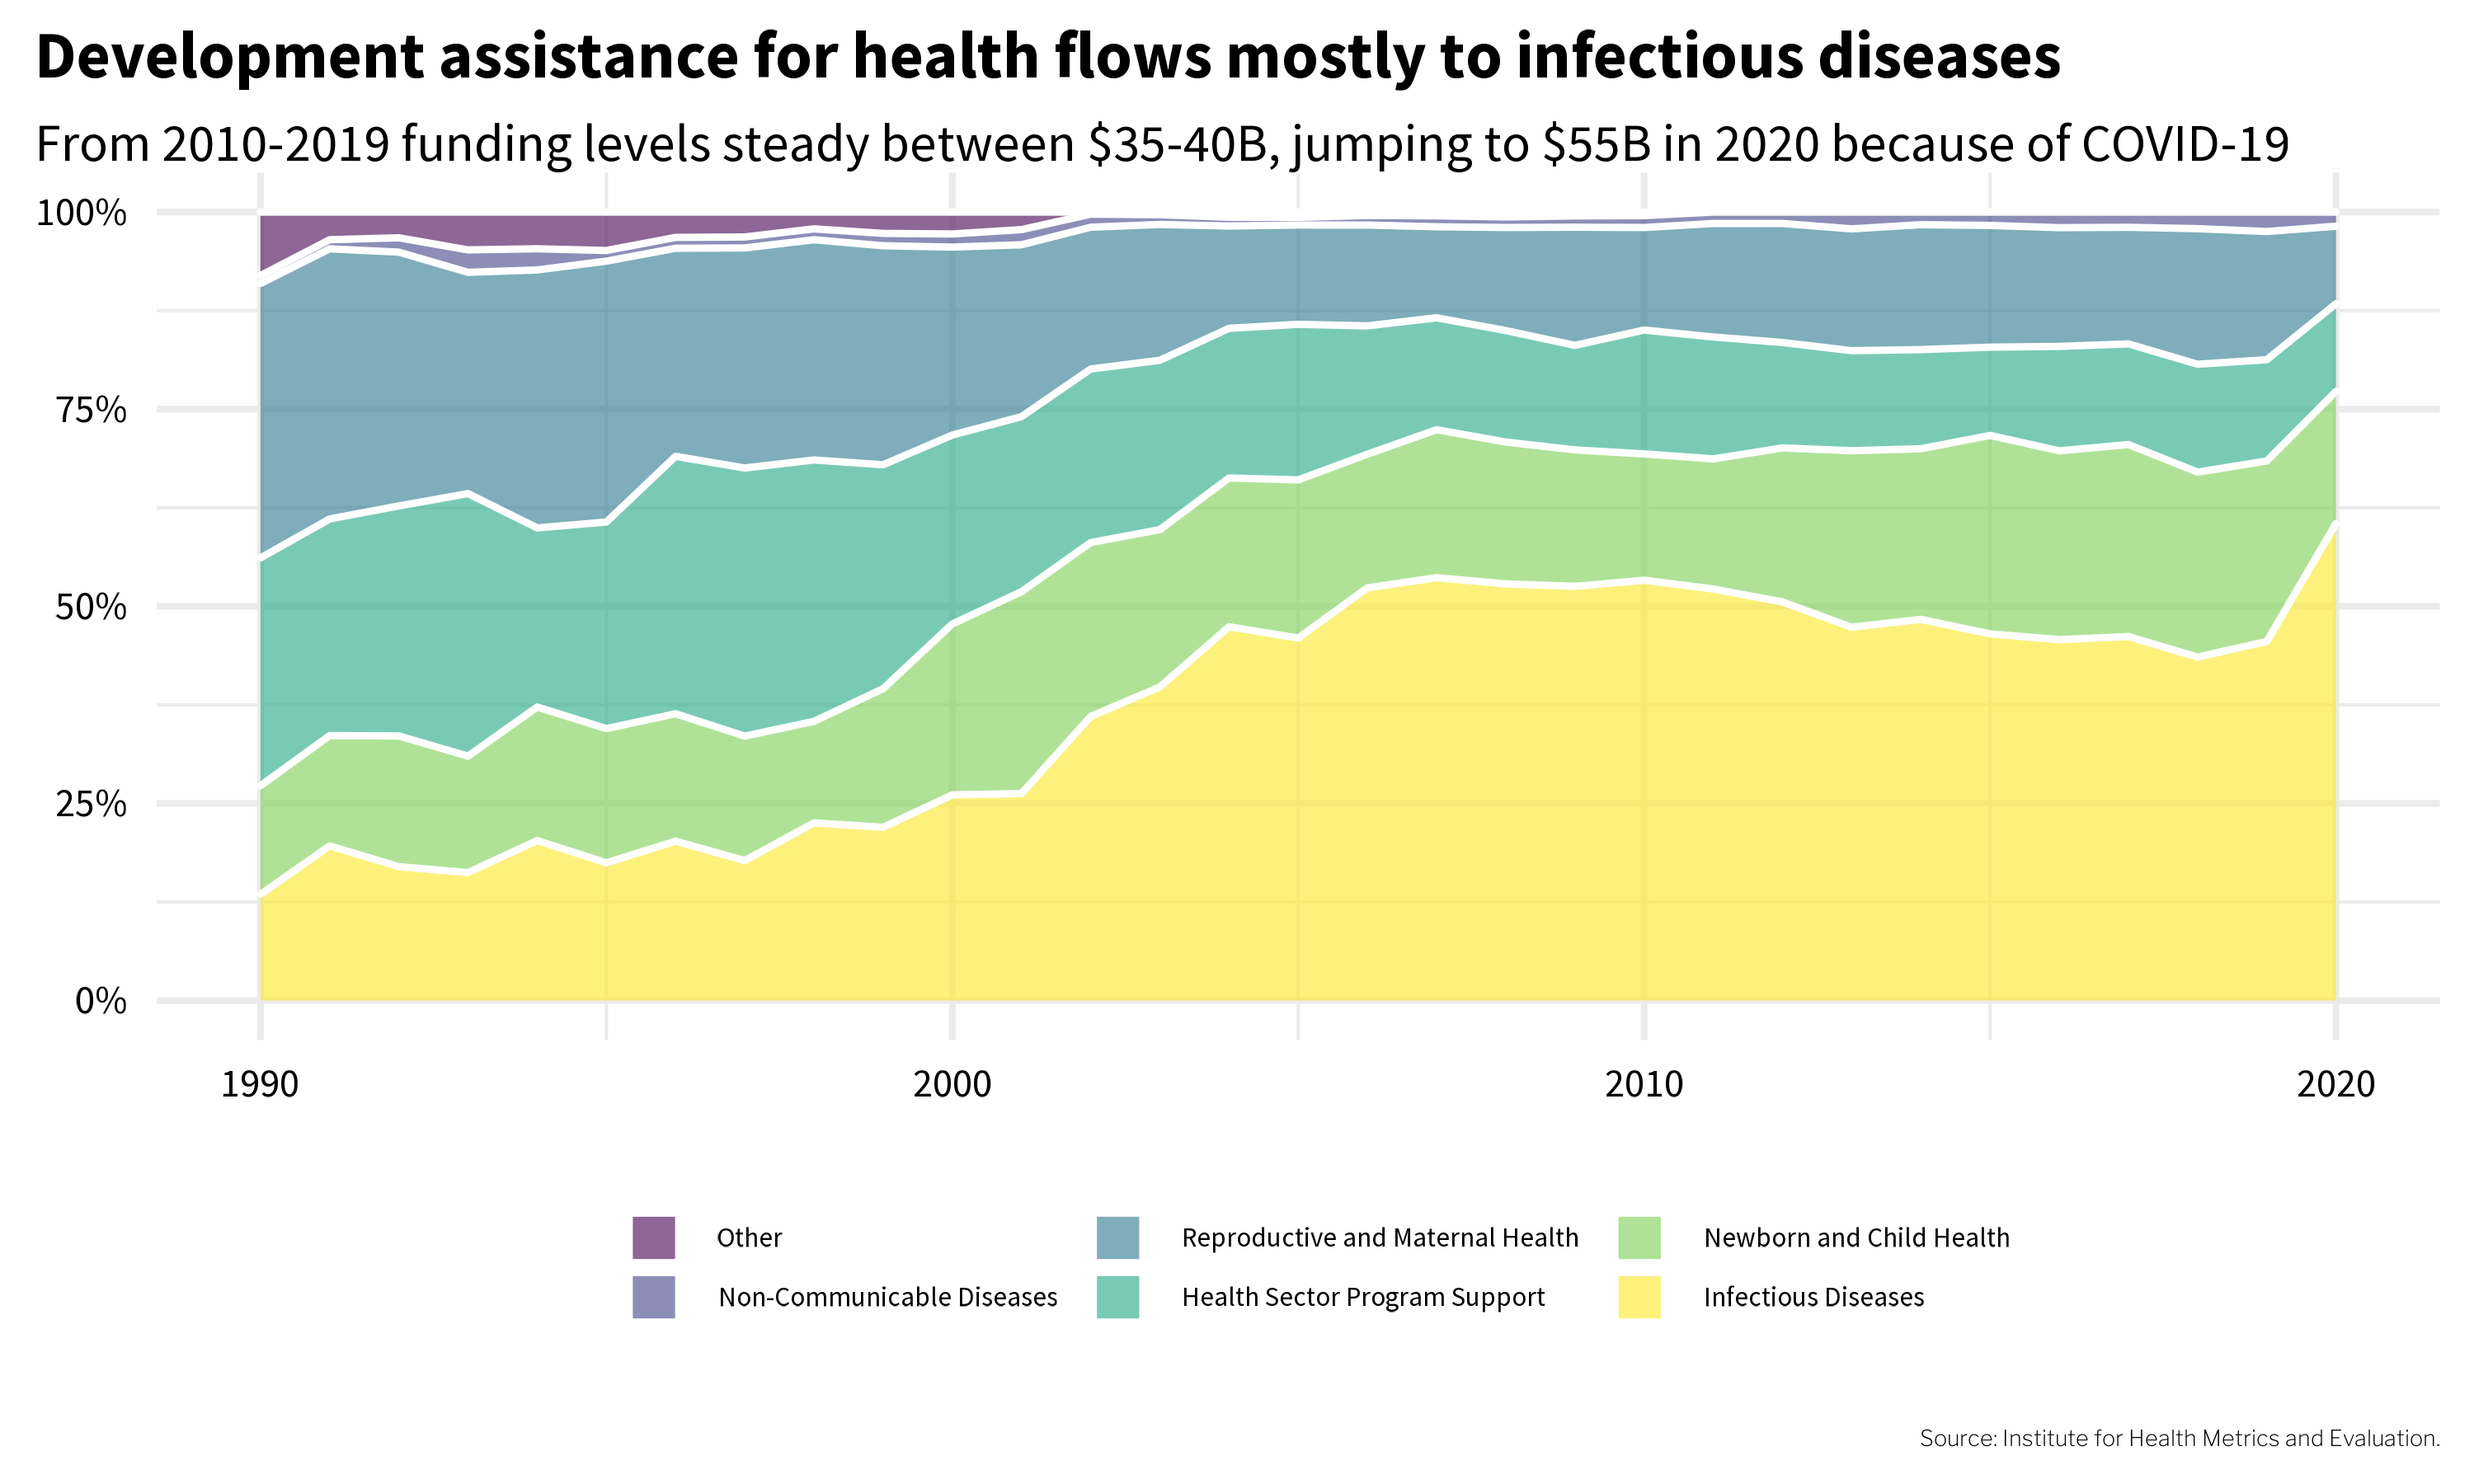
\includegraphics{images/figures/dah.png}

}

\caption{Development assistance for health by health focus area, 1990 to
2000.}

\end{figure}

Development assistance for health includes funded research, but it's not
inclusive of all research in low- and middle-income countries (e.g.,
does not include domestic spending on research). Nor does it capture
research on global health issues in wealthy nations. Inequities in
health exist everywhere, so by definition global health research is a
broad domain. It's difficult to put a dollar amount on the enterprise as
a whole. A 2013 analysis estimated that the global investment in health
research and development (R\&D) topped \$300 billion (in 2021
dollars).{[}@rottingen:2013{]}

According to this analysis, most investments in health R\&D come from
private industry (60\%), with the rest coming from the public sector
(30\%) and other sources (10\%). Very little money is directed to
pharmaceutical products and technologies for global health priorities
that disproportionately affect poor countries---less than \$4 billion in
2019.{[}@policycures{]} In this 2019 accounting, public and
philanthropic funders provided almost 90\% of the money. The two leading
funders were the United States National Institutes of Health (44\%) and
the Bill and Melinda Gates Foundation (16\%), contributing nearly
two-thirds of all research dollars between them.

The model for investments in R\&D for health is funding from the rich,
to the rich, (mostly) for the rich.

\hypertarget{who-sets-the-agenda-and-conducts-global-health-research}{%
\subsection{Who Sets the Agenda and Conducts Global Health
Research?}\label{who-sets-the-agenda-and-conducts-global-health-research}}

This is important context because funders have an outsized role in
setting the research agenda.{[}@sridhar:2012{]} Outside of industry,
researchers depend primarily on grants to fund their work. As nearly all
global health research funding comes from governments and philanthropies
in high-income countries, the global health research agenda is set in
large part by the wealthy.{[}@ii:2018{]}

The global health research agenda is also, in large part, carried out by
the wealthy. Only a fraction of 1\% of funding for biomedical research
goes \emph{directly} to recipients in low-income countries.{[}@whoob{]}
In-country researchers too often only play the role of partner or
collaborator, rather than principal investigator, if even
consulted.{[}@kyobutungi:2021{]} We'll revisit these power imbalances,
and what can be done to chart a more equitable and inclusive course for
global health research, in the next chapter.

\hypertarget{where-is-global-health-research-published}{%
\subsection{Where is Global Health Research
Published?}\label{where-is-global-health-research-published}}

\begin{Shaded}
\begin{Highlighting}[]
\FunctionTok{cat}\NormalTok{(tufte}\SpecialCharTok{::}\FunctionTok{margin\_note}\NormalTok{(}\StringTok{"}\SpecialCharTok{\textbackslash{}\textbackslash{}}\StringTok{faIcon\{youtube\} See how editors at The Lancet approach publishing global health research at }\SpecialCharTok{\textbackslash{}\textbackslash{}}\StringTok{href\{http://ghr.link/lan\}\{}\SpecialCharTok{\textbackslash{}\textbackslash{}}\StringTok{footnotesize}\SpecialCharTok{\textbackslash{}\textbackslash{}}\StringTok{texttt\{ghr.link/lan\}\}."}\NormalTok{))}
\end{Highlighting}
\end{Shaded}

\marginnote{\faIcon{youtube} See how editors at The Lancet approach publishing global health research at \href{http://ghr.link/lan}{\footnotesize\texttt{ghr.link/lan}}.}

\begin{Shaded}
\begin{Highlighting}[]
\NormalTok{knitr}\SpecialCharTok{::}\FunctionTok{include\_graphics}\NormalTok{(}\StringTok{"images/QR\_lan.png"}\NormalTok{)}
\end{Highlighting}
\end{Shaded}

\begin{figure}[H]

{\centering 
\includegraphics[width=0.2\textwidth,height=\textheight]{images/QR_lan.png}

}

\end{figure}

\begin{Shaded}
\begin{Highlighting}[]
\FunctionTok{cat}\NormalTok{(tufte}\SpecialCharTok{::}\FunctionTok{margin\_note}\NormalTok{(}\StringTok{"\textless{}iframe width=\textquotesingle{}300\textquotesingle{} height=\textquotesingle{}169\textquotesingle{} src=\textquotesingle{}https://www.youtube.com/embed/HN6zpQGvkSA\textquotesingle{} frameborder=\textquotesingle{}0\textquotesingle{} allow=\textquotesingle{}accelerometer; autoplay; encrypted{-}media; gyroscope; picture{-}in{-}picture\textquotesingle{} allowfullscreen\textgreater{}\textless{}/iframe\textgreater{}Editors at The Lancet discuss publishing global health research."}\NormalTok{))}
\end{Highlighting}
\end{Shaded}

Global health research is published in medical journals (e.g., \emph{The
Lancet}, \emph{JAMA}), general science journals (e.g., \emph{Science},
\emph{Nature}, \emph{PLOS ONE}), discipline-specific journals (e.g.,
\emph{The Journal of Immunology}, \emph{Epidemiology}), and
disease-specific journals (e.g., \emph{AIDS}, \emph{Malaria Journal}).
Journals specializing in global health research include \emph{The Lancet
Global Health}, \emph{BMJ Global Health}, \emph{Global Health: Science
and Practice}, and \emph{PLOS Global Public Health}.



\end{document}
